\documentclass[UTF8]{ctexart}
\usepackage{ctex}
\usepackage{graphicx}
\usepackage{color}
\usepackage{xcolor}
\usepackage{listings}
\usepackage{float}
\usepackage{amsmath}
\usepackage{tikz}
\usepackage{pgfplots}
\usepackage{fancyhdr}
\usepackage{mdframed}
\usepackage{caption}
\usepackage{ booktabs}
\usepackage{makecell}
\usepackage{amsthm}
\usepackage{hyperref }
\usepackage{ pgffor }
\usepackage{caption}
\usepackage{subcaption}
\usepackage{afterpage}
\usepackage{geometry} % 页面边距设置
\geometry{left=2.5cm, right=2.5cm, top=2.5cm, bottom=2.5cm}
%================================================================================================================%
\begin{document}


% 插入图片,调整宽度为页面宽度
\begin{center}
    
\includegraphics[width=\textwidth]{o} % 替换为您的图片文件名
\end{center}

% 定义标题
\begin{center}
    \huge\textbf{第二周实验报告}
\end{center}

% 定义作者
\begin{center}
    \huge\textbf{於佳杰}
\end{center}
% 以下内容将从下一页开始
\newpage

\title{第二周实验报告}
\author{於佳杰}
\date{2024 年 9 月 3 日}
\maketitle

\pagenumbering{arabic}
\tableofcontents
\newpage
\pagenumbering{arabic}

\pagestyle{fancy}
\fancyhf{}
\renewcommand{\headrulewidth}{1pt}
\renewcommand{\footrulewidth}{1pt}
\fancyhead[L]{
\includegraphics[width=1.5cm]{okkl}} % 确保图片路径正确
\fancyhead[C]{\rightmark}
\fancyfoot[C]{\thepage}
\fancyhead[R]{\thepage}


% 1实验目的================================================================================================%

\section{实验目的}
{\color{red}掌握Shell工具和脚本、编辑器(Vim)和数据整理;}
% 2实例展示================================================================================================%
\section{实例展示}

%Shell工具和脚本=========================================================================%
  \subsection{Shell}
  {\color{blue}LaTex命令展示}



%1.1.1列表==================================================%
\subsubsection{读取 man ls 并编写一个命令,按以下方式列出文件ls}

\begin{enumerate}
  \item 包括所有文件,包括隐藏文件\\
尺寸以人类可读的格式列出(例如 454M 而不是 454279954)\\
文件按新近度排序\\
输出是彩色的
  \begin{itemize}
  \item 命令展示
  \begin{verbatim}
  ls -lah --sort=time --color=auto

    
  \end{verbatim}

  \item 效果展示
  \begin{figure}[H]
    \centering
    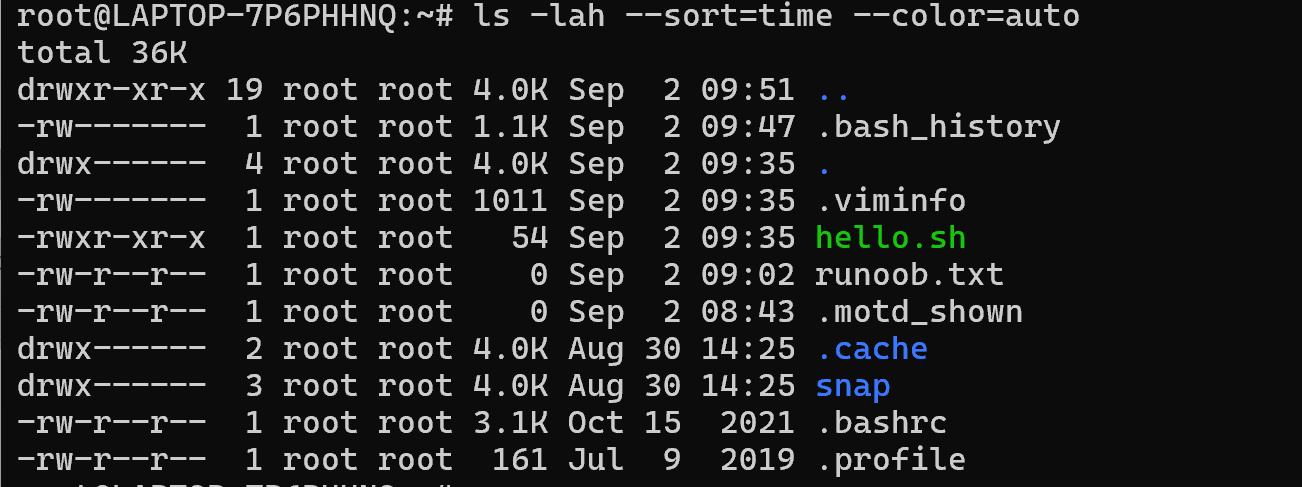
\includegraphics[width=\textwidth]{1} % 确保文件名正确
    \caption{效果展示}
  
  \end{figure}
\end{itemize}
\end{enumerate}
%1.1.2表格==================================================%
\subsubsection{ 编写一个 bash 脚本}

\begin{enumerate}
  \item  假设您有一个很少失败的命令。为了调试它,您需要捕获其输出,但运行失败可能很耗时。\\该脚本运行以下脚本,直到它失败,并将其标准输出和错误流捕获到文件中,并在最后打印所有内容。 如果还可以报告脚本失败所需的运行次数,则加分。
  \begin{itemize}
  \item 命令展示
  \begin{verbatim}
 #!/usr/bin/env bash

# 保存输出的文件
output_file="output.log"
# 初始化计数器
count=0

# 清空之前的日志文件
> "$output_file"

# 循环执行,直到脚本失败
while true; do
    # 增加计数器
    ((count++))
    
    # 执行目标脚本,捕获输出和错误,并附加到日志文件中
    ./rare_fail.sh >> "$output_file" 2>&1
    
    # 检查上一个命令的退出状态
    if [[ $? -ne 0 ]]; then
        # 记录失败信息
        echo "Script failed after $count attempts." >> "$output_file"
        # 打印日志文件内容
        cat "$output_file"
        # 退出循环
        break
    fi
done


    
  \end{verbatim}

  \item 效果展示
  \begin{figure}[H]
    \centering
    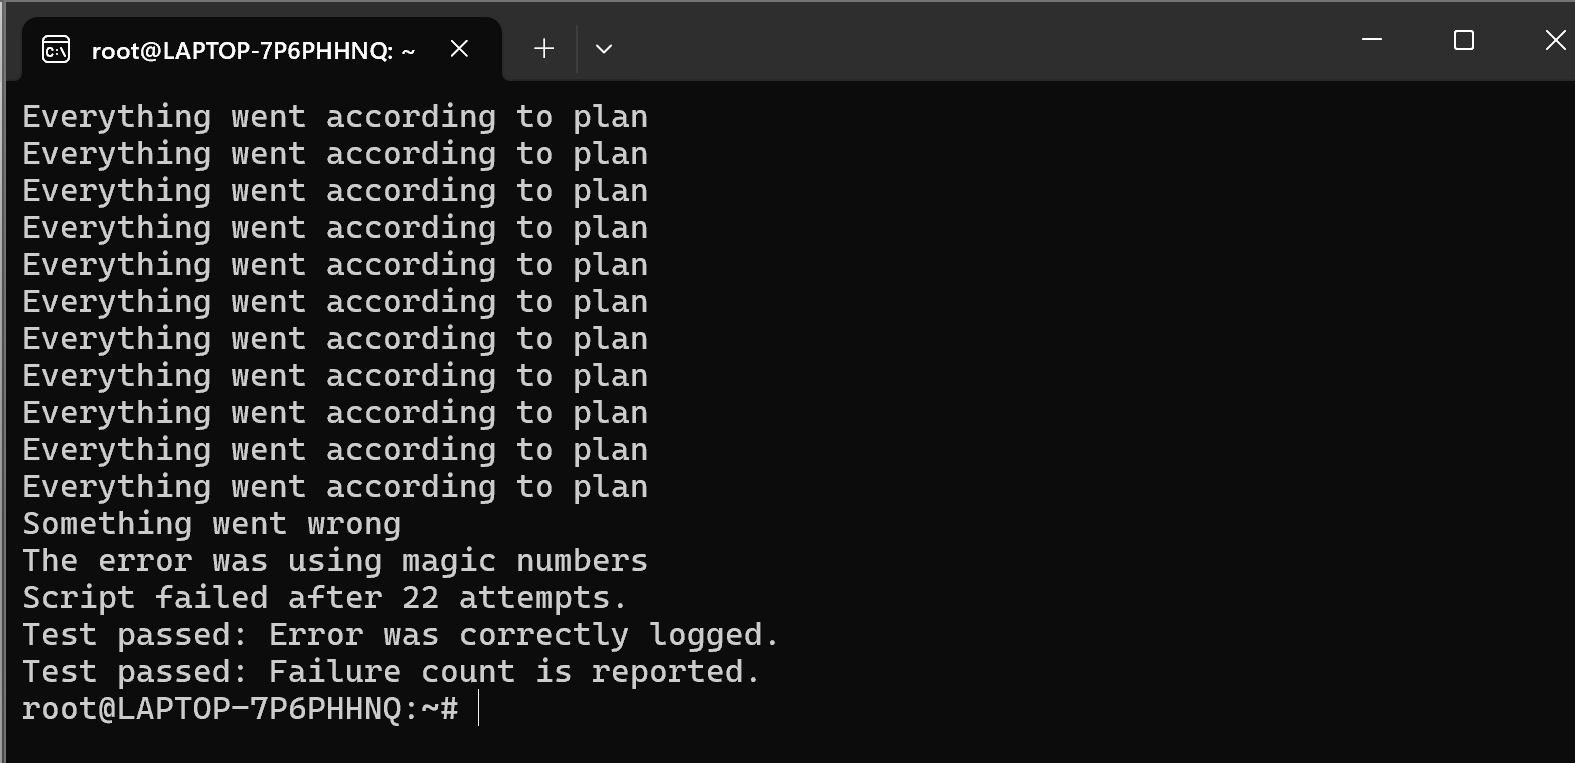
\includegraphics[width=\textwidth]{2} % 确保文件名正确
     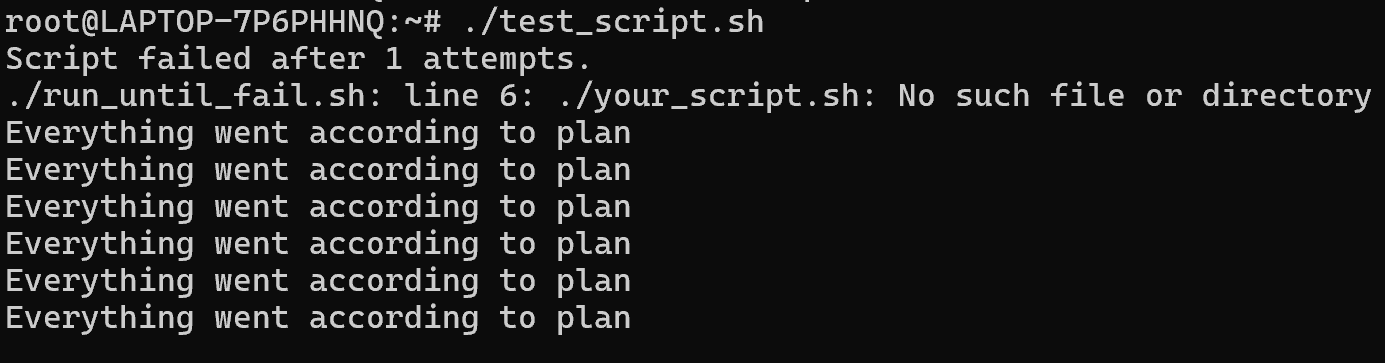
\includegraphics[width=\textwidth]{3} % 确保文件名正确
    \caption{效果展示}
  
  \end{figure}
\end{itemize}
\end{enumerate}




%1.1.3图表==================================================%
\subsubsection{编写一个命令}

\begin{enumerate}
  \item 以递归方式查找文件夹中的所有 HTML 文件,并使用它们创建 zip。请注意,即使文件包含空格,您的命令也应该有效(提示:检查标志)。-dxargs
  \begin{itemize}
  \item 命令展示
  \begin{verbatim}
 find . -type f -name "*.html" -print0 | xargs -0 zip html_files.zip


    
  \end{verbatim}

  \item 效果展示
  \begin{figure}[H]
    \centering
    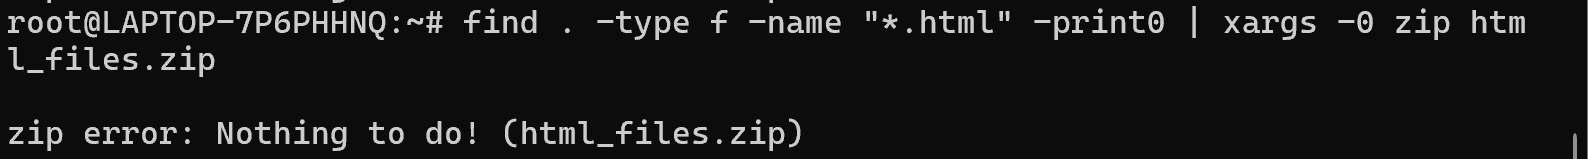
\includegraphics[width=\textwidth]{4} % 确保文件名正确
    \caption{效果展示}
  
  \end{figure}
\end{itemize}
\end{enumerate}








%1.1.4基本数学公式==================================================%

\subsubsection{编写命令或脚本}

\begin{enumerate}
  \item 编写命令或脚本以递归方式查找目录中最近修改的文件。更一般地说,您能否按新近度列出所有文件?
  \begin{itemize}
  \item 命令展示
  \begin{verbatim}

 #!/bin/bash

# 目录路径
DIR=${1:-/root}

# 使用 find 列出所有文件按修改时间排序
find "$DIR" -type f -printf "%T@ %p\n" | sort -n -r | while read -r line; do
    timestamp=$(echo "$line" | cut -d' ' -f1)
    filepath=$(echo "$line" | cut -d' ' -f2-)
    mod_time=$(date -d @"$timestamp" "+%Y-%m-%d %H:%M:%S")
    echo "$mod_time $filepath"
done | head -n 10

    
  \end{verbatim}

  \item 效果展示
  \begin{figure}[H]
    \centering
    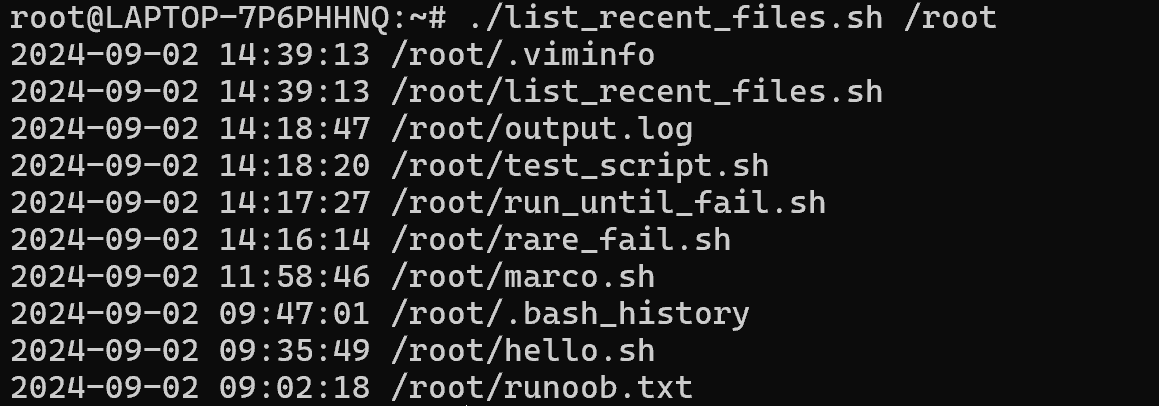
\includegraphics[width=\textwidth]{5} % 确保文件名正确
    \caption{效果展示}
  
  \end{figure}
\end{itemize}
\end{enumerate}

%1.1.5画图==================================================%
\subsubsection{自动化数据库备份}

\begin{enumerate}
 \item 用脚本实现自动化数据库备份
  \begin{itemize}
  \item 命令展示

  \begin{verbatim}
   
  \begin{itemize}
  #!/bin/bash

# 定义数据库连接信息
DB_HOST="localhost"
DB_USER="user"
DB_PASS="password"
DB_NAME="database"

# 定义备份存放目录
BACKUP_DIR="/path/to/db_backup"

# 获取当前日期以用于创建唯一的备份文件名
DATE=$(date +%Y%m%d%H%M%S)

# 创建备份存放目录(如果不存在)
mkdir -p "$BACKUP_DIR"

# 备份数据库并保存为.sql文件
BACKUP_FILE="$BACKUP_DIR/$DB_NAME-$DATE.sql"

# 使用mysqldump执行数据库备份
mysqldump -h "$DB_HOST" -u "$DB_USER" -p"$DB_PASS" "$DB_NAME" > "$BACKUP_FILE"

# 检查备份是否成功
if [ $? -eq 0 ]; then
  echo "数据库备份成功,文件存储为:$BACKUP_FILE"
else
  echo "数据库备份失败"
fi

    
  \end{verbatim}

  \item 效果展示
  \begin{figure}[H]
    \centering
    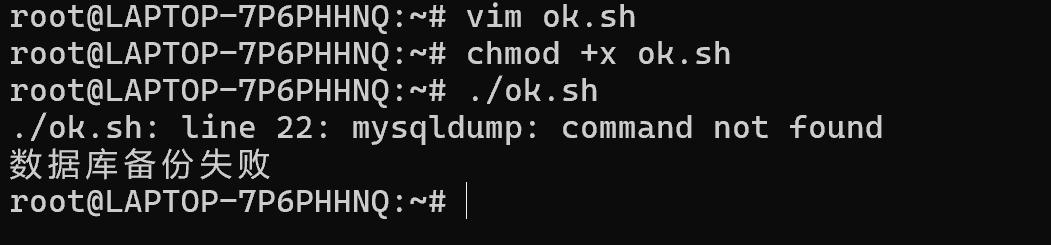
\includegraphics[width=\textwidth]{6} % 确保文件名正确
    \caption{效果展示}
  
  \end{figure}
\end{itemize}
\end{enumerate}
%1.1.6画函数图像==================================================%

\subsubsection{批量重命名文件}

\begin{enumerate}
  \item 用脚本实现批量重命名文件

  \begin{itemize}
  \item 命令展示
  \begin{verbatim}
#!/bin/bash

# 定义要处理的文件目录
TARGET_DIR="/path/to/files"

# 定义文件的新前缀
NEW_PREFIX="newname"

# 初始化计数器
COUNT=1

# 遍历目录中的所有文件
for FILE in "$TARGET_DIR"/*; do
  # 获取文件的扩展名
  EXT="${FILE##*.}"
  
  # 构建新的文件名
  NEW_NAME="$TARGET_DIR/$NEW_PREFIX-$COUNT.$EXT"
  
  # 重命名文件
  mv "$FILE" "$NEW_NAME"
  
  # 输出重命名信息
  echo "重命名:$FILE -> $NEW_NAME"
  
  # 递增计数器
  ((COUNT++))
done


    
  \end{verbatim}

  \item 效果展示
  \begin{figure}[H]
    \centering
    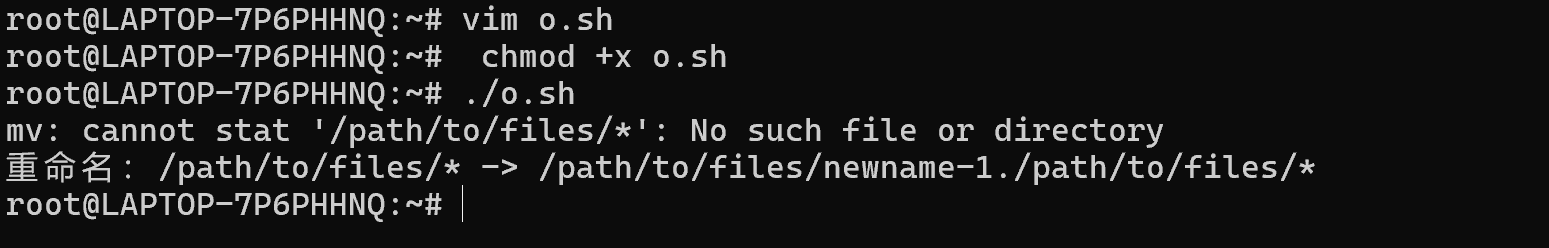
\includegraphics[width=\textwidth]{7} % 确保文件名正确
    \caption{效果展示}
  
  \end{figure}
\end{itemize}
\end{enumerate}
%1.1.7矩阵==================================================%
\subsubsection{检测并自动修复缺失的软件包}

\begin{enumerate}
  \item 用脚本实现检测并自动修复缺失的软件包
  \begin{itemize}
  \item 命令展示
  \begin{verbatim}
#!/bin/bash

# 定义需要的包列表
REQUIRED_PACKAGES=("curl" "git" "vim" "htop")

# 遍历每个包以检查是否已安装
for PACKAGE in "${REQUIRED_PACKAGES[@]}"; do
  # 检查包是否已安装
  dpkg -s "$PACKAGE" &> /dev/null
  
  # 如果包未安装,则进行安装
  if [ $? -ne 0 ]; then
    echo "$PACKAGE 未安装,正在安装..."
    sudo apt-get install -y "$PACKAGE"
    
    # 检查安装是否成功
    if [ $? -eq 0 ]; then
      echo "$PACKAGE 安装成功"
    else
      echo "$PACKAGE 安装失败"
    fi
  else
    echo "$PACKAGE 已安装"
  fi
done


    
  \end{verbatim}

  \item 效果展示
  \begin{figure}[H]
    \centering
    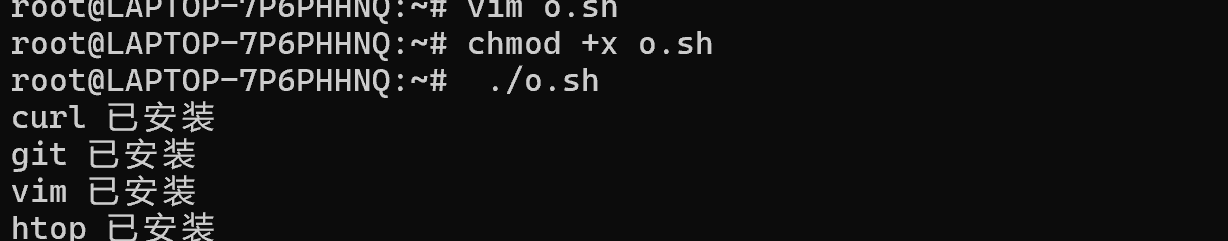
\includegraphics[width=\textwidth]{8} % 确保文件名正确
    \caption{效果展示}
  
  \end{figure}
\end{itemize}
\end{enumerate}
%1.1.8页眉页脚==================================================%
\subsubsection{自动化日志文件轮转}

\begin{enumerate}
  \item 用脚本实现
  \begin{itemize}
  \item 命令展示
  \begin{verbatim}
 #!/bin/bash

# 定义日志文件目录和轮转后的存放目录
LOG_DIR="/path/to/logs"
ARCHIVE_DIR="/path/to/log_archive"

# 获取当前日期以用于创建唯一的存档目录
DATE=$(date +%Y%m%d)

# 创建存档目录(如果不存在)
mkdir -p "$ARCHIVE_DIR/$DATE"

# 遍历日志目录中的所有日志文件
for LOG_FILE in "$LOG_DIR"/*.log; do
  # 获取文件名
  FILE_NAME=$(basename "$LOG_FILE")
  
  # 压缩日志文件并移动到存档目录
  gzip -c "$LOG_FILE" > "$ARCHIVE_DIR/$DATE/$FILE_NAME.gz"
  
  # 清空原日志文件
  cat /dev/null > "$LOG_FILE"
  
  # 输出操作信息
  echo "已轮转日志文件:$LOG_FILE"
done

    
  \end{verbatim}

  \item 效果展示
  \begin{figure}[H]
    \centering
    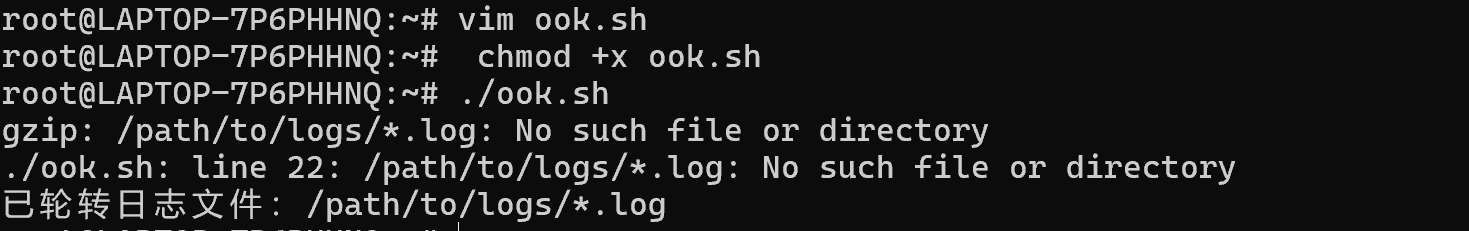
\includegraphics[width=\textwidth]{9} % 确保文件名正确
    \caption{效果展示}
  
  \end{figure}
\end{itemize}
\end{enumerate}

%1.1.9并排图==================================================%
\subsubsection{自动化用户账户创建}

\begin{enumerate}
  \item 用脚本实现自动化用户账户创建
  \begin{itemize}
  \item 命令展示
  \begin{verbatim}
#!/bin/bash

# 检查是否以root身份运行
if [ "$(id -u)" -ne 0 ]; then
  echo "请以root权限运行此脚本"
  exit 1
fi

# 从文件读取用户列表
USER_FILE="/path/to/userlist.txt"

# 检查用户列表文件是否存在
if [ ! -f "$USER_FILE" ]; then
  echo "用户列表文件不存在"
  exit 1
fi

# 遍历文件中的每一行
while IFS= read -r USER; do
  # 创建用户并设置默认密码
  useradd "$USER"
  echo "$USER:defaultpassword" | chpasswd
  
  # 检查用户是否创建成功
  if [ $? -eq 0 ]; then
    echo "用户 $USER 创建成功"
  else
    echo "用户 $USER 创建失败"
  fi
done < "$USER_FILE"


    
  \end{verbatim}

  \item 效果展示
  \begin{figure}[H]
    \centering
    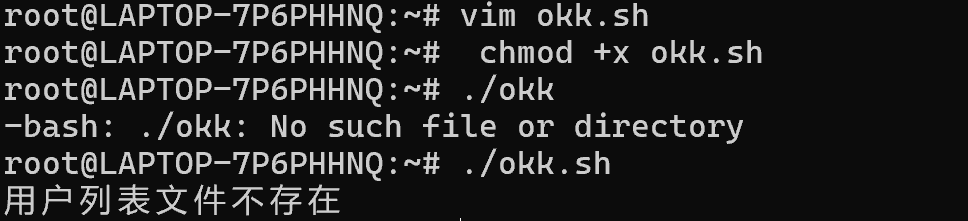
\includegraphics[width=\textwidth]{10} % 确保文件名正确
    \caption{效果展示}
  
  \end{figure}
\end{itemize}
\end{enumerate}
%1.1.10三线表==================================================%
\subsubsection{自动化系统更新和清理}

\begin{enumerate}
  \item 用脚本实现自动化系统更新和清理
  \begin{itemize}
  \item 命令展示
  \begin{verbatim}
#!/bin/bash

# 检查是否以root身份运行
if [ "$(id -u)" -ne 0 ]; then
  echo "请以root权限运行此脚本"
  exit 1
fi

# 更新包列表并升级系统
echo "正在更新系统..."
apt-get update && apt-get upgrade -y

# 自动清理不再需要的软件包和缓存
echo "正在清理系统..."
apt-get autoremove -y
apt-get autoclean

# 检查更新和清理是否成功
if [ $? -eq 0 ]; then
  echo "系统更新和清理完成"
else
  echo "系统更新或清理失败"
fi



    
  \end{verbatim}

  \item 效果展示
  \begin{figure}[H]
    \centering
    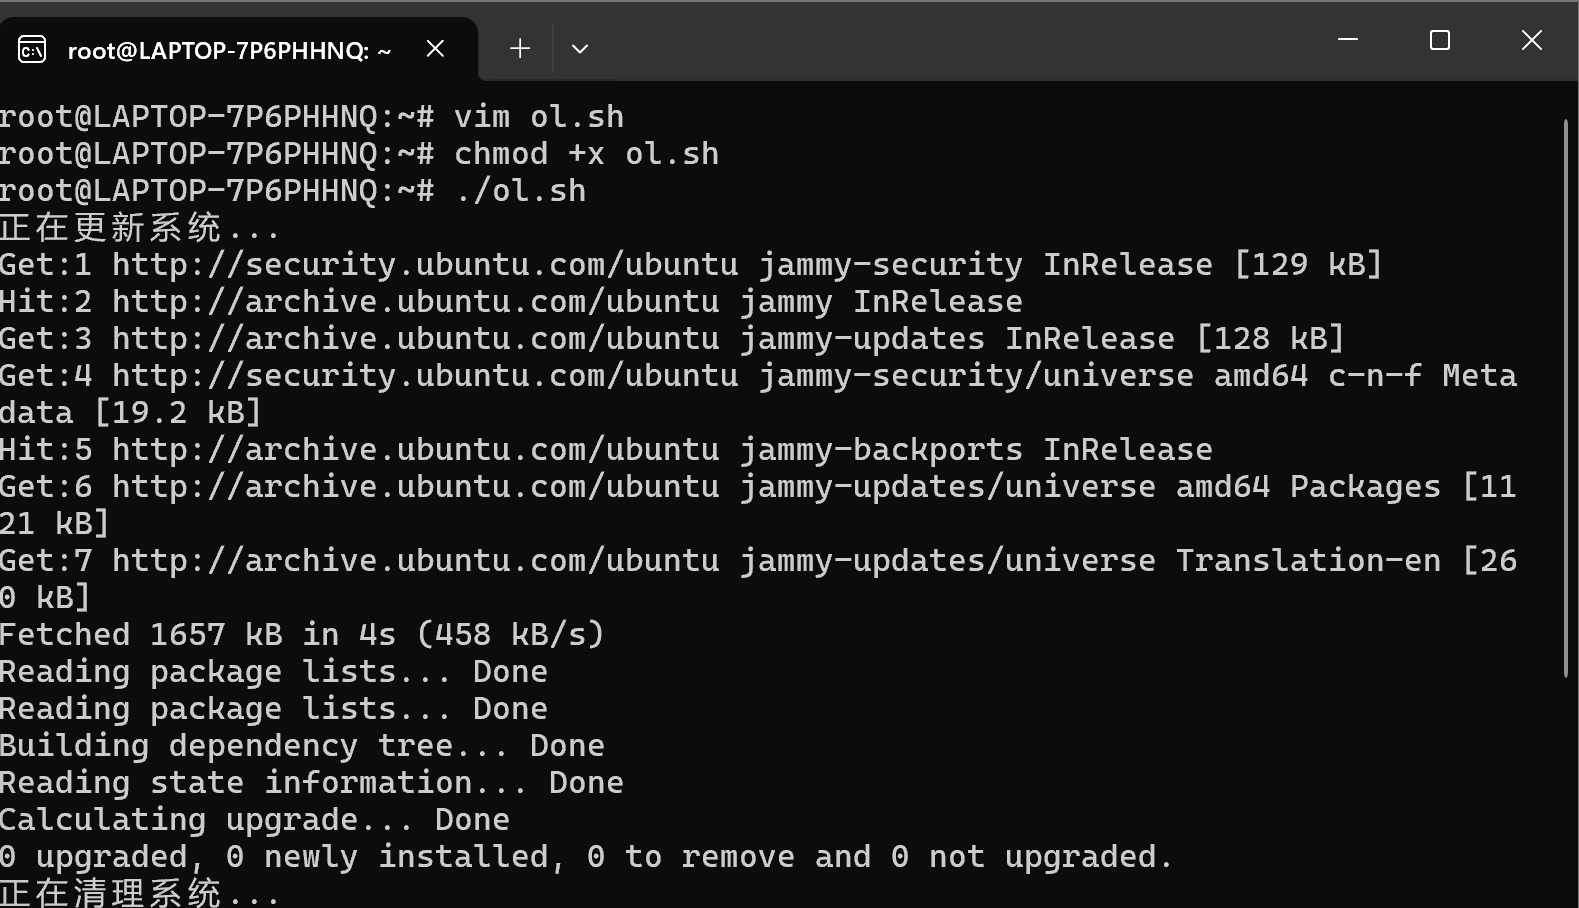
\includegraphics[width=\textwidth]{11}

    \caption{效果展示}
  
  \end{figure}
  
  \begin{figure}[H]
    \centering
   
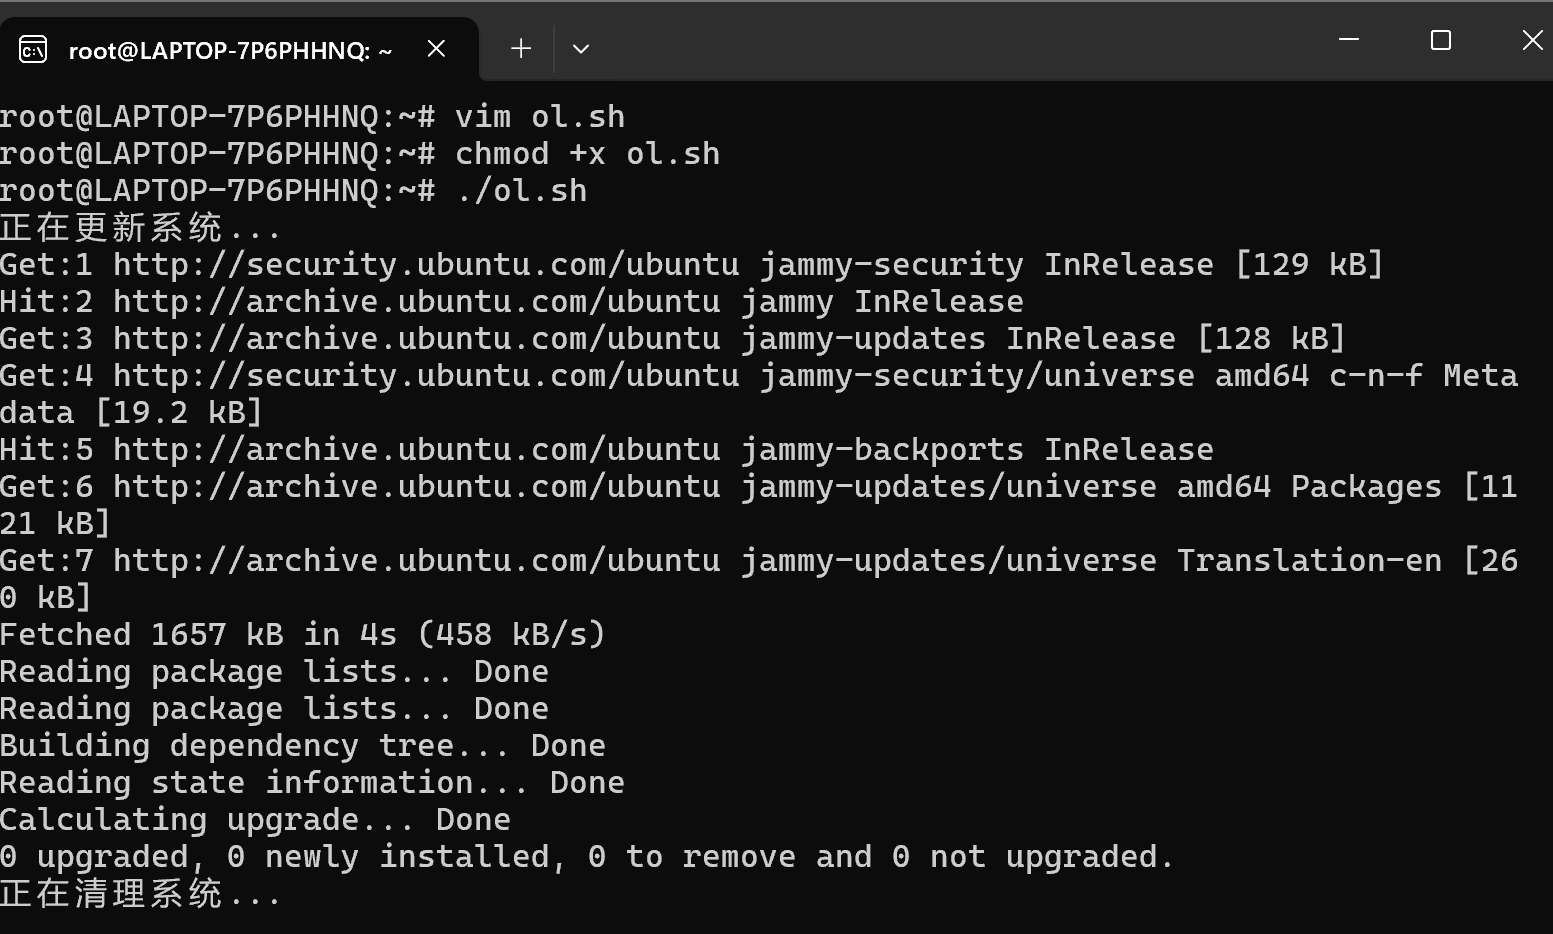
\includegraphics[width=\textwidth]{111} % 确保文件名正确
    \caption{效果展示}
  
  \end{figure}
\end{itemize}
\end{enumerate}
%1.1.11嵌套表格==================================================%
\subsubsection{自动化磁盘使用情况报告}

\begin{enumerate}
  \item 这个脚本会生成一份磁盘使用情况报告,并发送到指定的电子邮件地址。

  \begin{itemize}
  \item 命令展示
  \begin{verbatim}
#!/bin/bash

# 定义报告文件和接收邮件的地址
REPORT_FILE="/home/user/disk_usage_report.txt"
EMAIL="example@example.com"

# 生成磁盘使用报告
df -h > "$REPORT_FILE"

# 使用mail命令发送报告
# 请确保系统安装并配置了mailutils或其他邮件工具
mail -s "磁盘使用情况报告" "$EMAIL" < "$REPORT_FILE"

# 检查邮件是否发送成功
if [ $? -eq 0 ]; then
  echo "磁盘使用报告已发送到 $EMAIL"
else
  echo "报告发送失败"
fi


    
  \end{verbatim}

  \item 效果展示
  \begin{figure}[H]
    \centering
    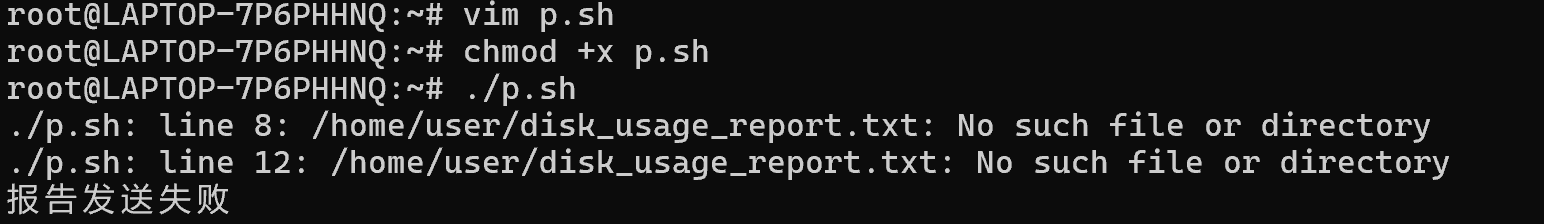
\includegraphics[width=\textwidth]{12} % 确保文件名正确
    \caption{效果展示}
  
  \end{figure}
\end{itemize}
\end{enumerate}
%1.1.12多行公式==================================================%
\subsubsection{自动化日志文件分析}

\begin{enumerate}
  \item 个脚本用来分析特定格式的日志文件,并生成一个错误报告
  \begin{itemize}
  \item 命令展示
  \begin{verbatim}
#!/bin/bash

# 定义日志文件路径和输出报告文件
LOG_FILE="/var/log/system.log"
REPORT_FILE="/home/user/error_report.txt"

# 清空之前的报告文件
> "$REPORT_FILE"

# 分析日志文件,并提取包含"ERROR"的行
echo "错误报告 - $(date)" >> "$REPORT_FILE"
echo "===================================" >> "$REPORT_FILE"
grep "ERROR" "$LOG_FILE" >> "$REPORT_FILE"

# 输出结果
if [ $? -eq 0 ]; then
  echo "错误报告已生成:$REPORT_FILE"
else
  echo "未在日志中发现错误。"
fi


    
  \end{verbatim}

  \item 效果展示
  \begin{figure}[H]
    \centering
    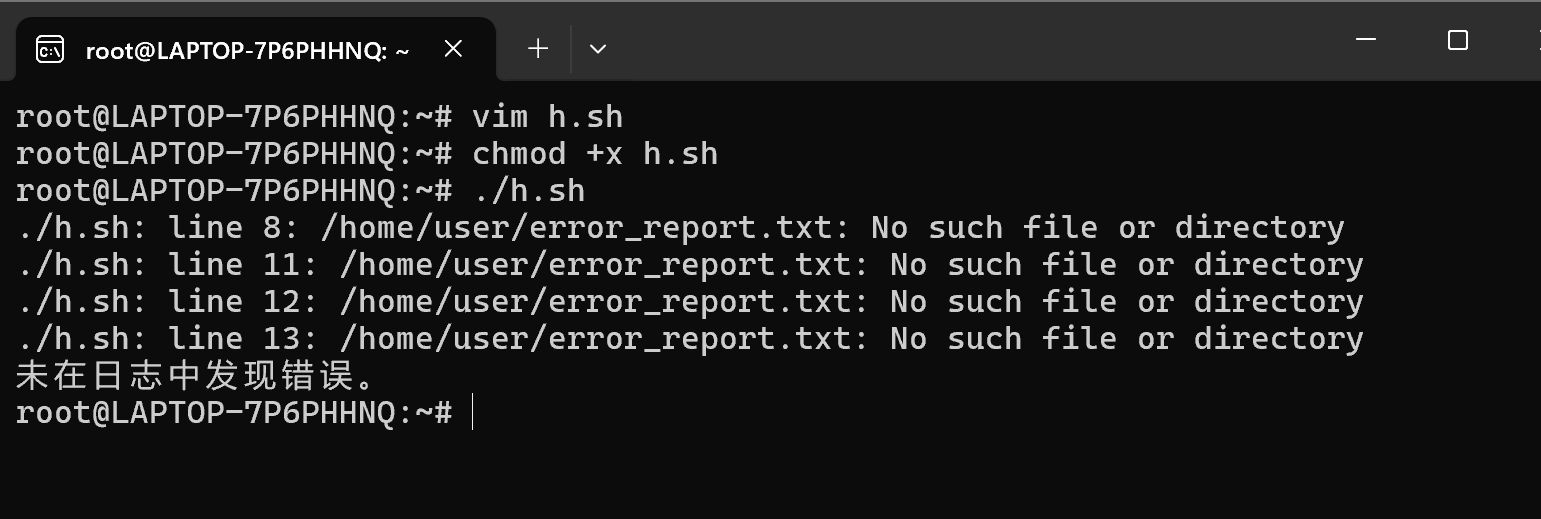
\includegraphics[width=\textwidth]{13} % 确保文件名正确
    \caption{效果展示}
  
  \end{figure}
\end{itemize}
\end{enumerate}
%1.1.13按等号对齐的多行公式==================================================%
\subsubsection{监控文件内容的实时变化}

\begin{enumerate}
  \item 监控文件内容的实时变化
输出是彩色的
  \begin{itemize}
  \item 命令展示
  \begin{verbatim}
    # 使用 tail 命令实时查看 "example.log" 文件的新内容
tail -f example.log
    
  \end{verbatim}

  \item 效果展示
  \begin{figure}[H]
    \centering
    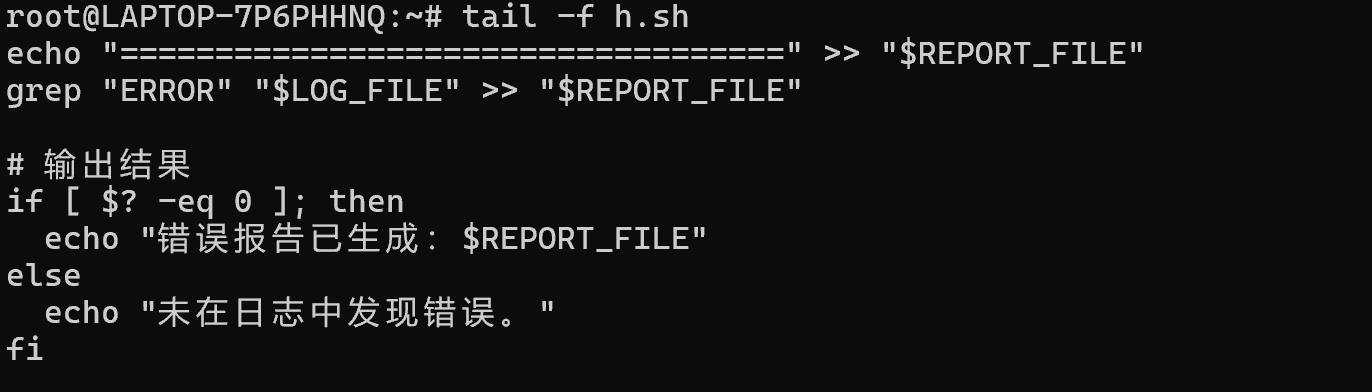
\includegraphics[width=\textwidth]{14} % 确保文件名正确
    \caption{效果展示}
  
  \end{figure}
\end{itemize}
\end{enumerate}
%1.1.14分段函数==================================================%
\subsubsection{统计目录下文件的行数}

\begin{enumerate}
  \item 统计目录下文件的行数
  \begin{itemize}
  \item 命令展示
  \begin{verbatim}

find . -type f -exec wc -l {} + | sort -n

    
  \end{verbatim}

  \item 效果展示
  \begin{figure}[H]
    \centering
    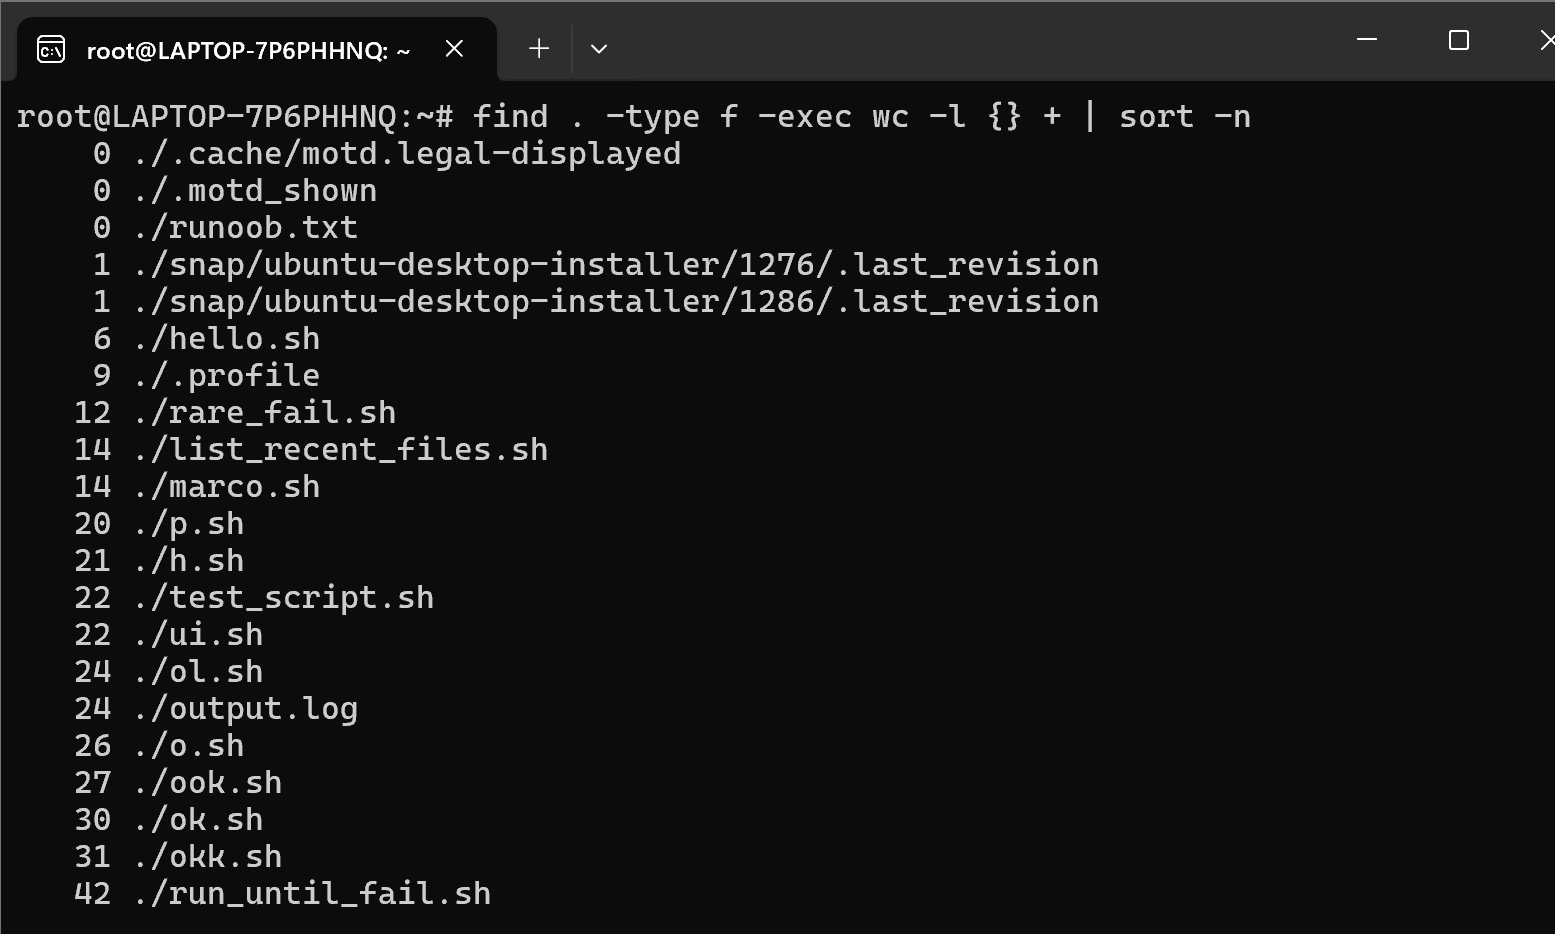
\includegraphics[width=\textwidth]{15}

    \caption{效果展示}
  
  \end{figure}
\begin{figure}[H]
    \centering
  
   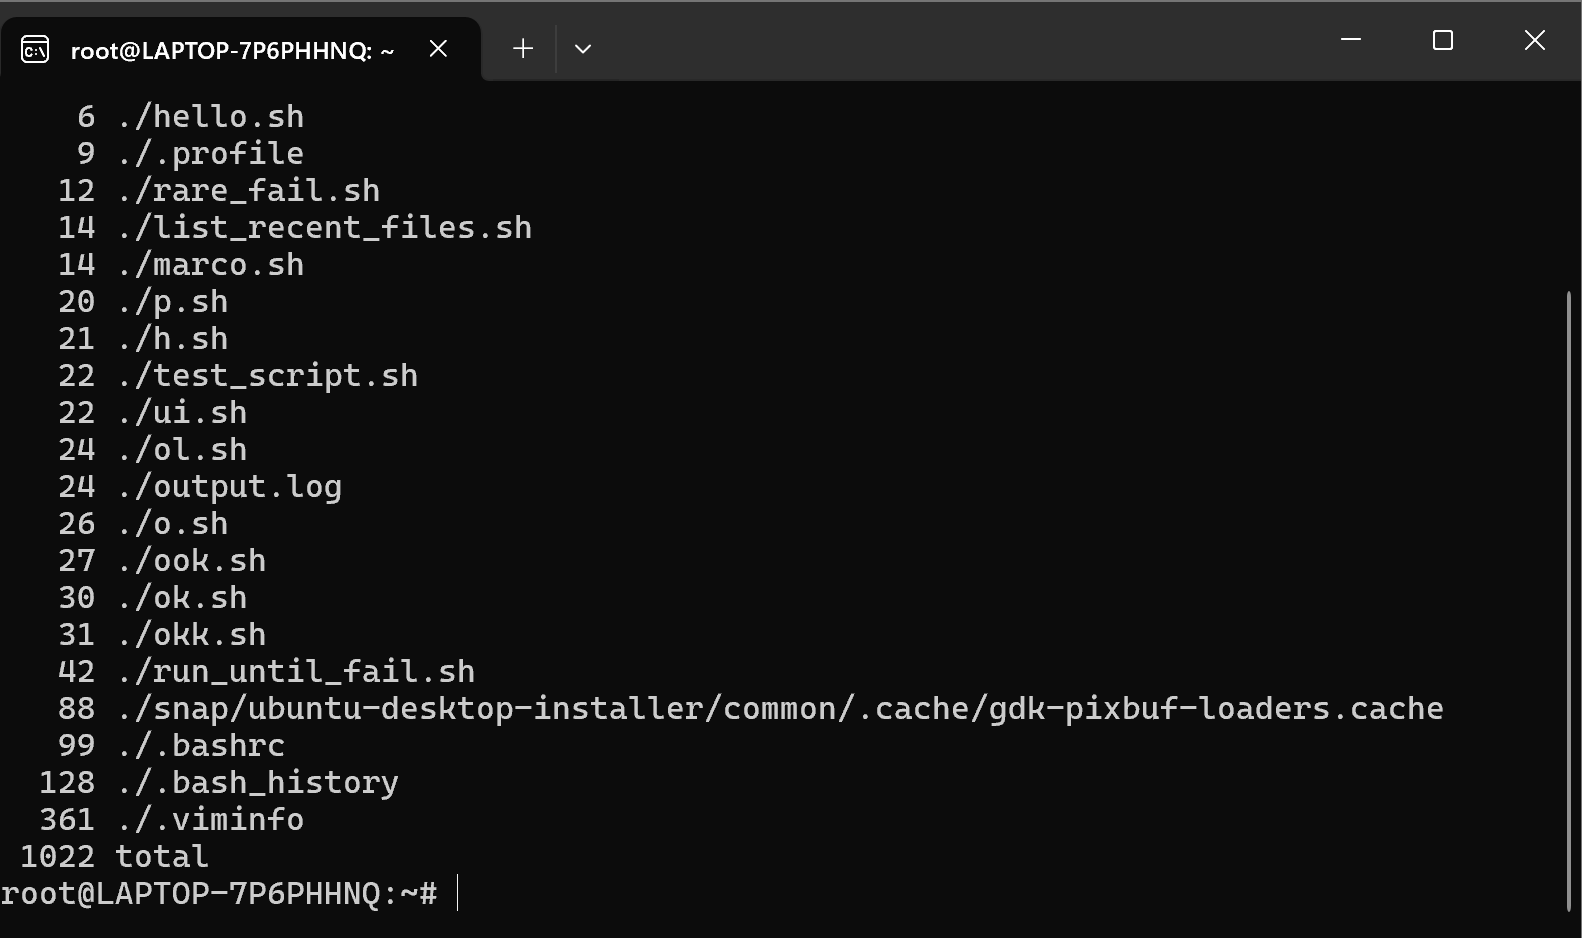
\includegraphics[width=\textwidth]{151}  % 确保文件名正确
    \caption{效果展示}
  
  \end{figure}
\end{itemize}
\end{enumerate}
%1.1.15 证明环境和证毕符号==================================================%
\subsubsection{显示文件的最后十行}

\begin{enumerate}
  \item 显示文件的最后十行
  \begin{itemize}
  \item 命令展示
  \begin{verbatim}
tail -n 10 filename.txt


    
  \end{verbatim}

  \item 效果展示
  \begin{figure}[H]
    \centering
    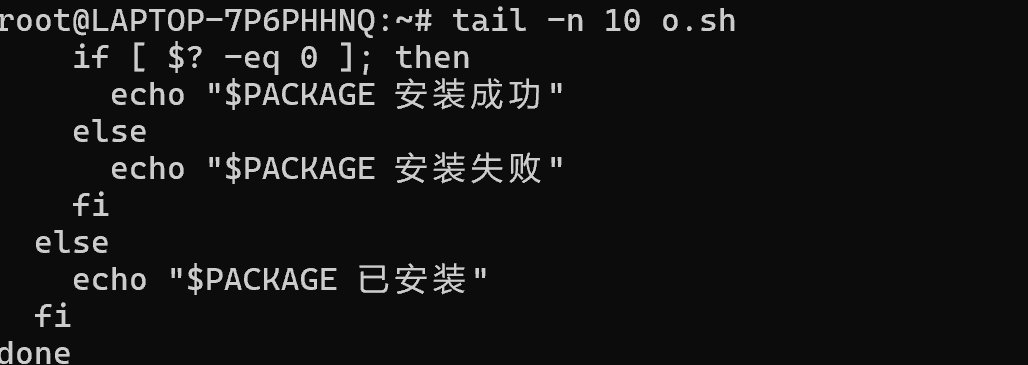
\includegraphics[width=\textwidth]{16} % 确保文件名正确
    \caption{效果展示}
  
  \end{figure}
\end{itemize}
\end{enumerate}
%1.1.16颜色的表达==================================================%
\subsubsection{自动化日志归档和清理}

\begin{enumerate}
  \item 脚本将特定目录中的日志文件归档并压缩,然后删除超过指定天数的归档文件。
  \begin{itemize}
  \item 命令展示
  \begin{verbatim}
 #!/bin/bash

# 定义日志文件目录和归档目录
LOG_DIR="/var/log/myapp"
ARCHIVE_DIR="/var/log/myapp/archive"
DAYS_TO_KEEP=30

# 创建归档目录(如果不存在)
mkdir -p "$ARCHIVE_DIR"

# 压缩并归档日志文件
for LOG_FILE in "$LOG_DIR"/*.log; do
  ARCHIVE_FILE="$ARCHIVE_DIR/$(basename "$LOG_FILE").$(date +%Y%m%d).gz"
  gzip -c "$LOG_FILE" > "$ARCHIVE_FILE"
  echo "已归档日志文件 $(basename "$LOG_FILE") 到 $ARCHIVE_FILE"
  echo "" > "$LOG_FILE"  # 清空原日志文件
done

# 删除超过指定天数的归档文件
find "$ARCHIVE_DIR" -type f -mtime +"$DAYS_TO_KEEP" -exec rm -f {} \;
echo "超过 $DAYS_TO_KEEP 天的归档文件已删除"

    
  \end{verbatim}

  \item 效果展示
  \begin{figure}[H]
    \centering
    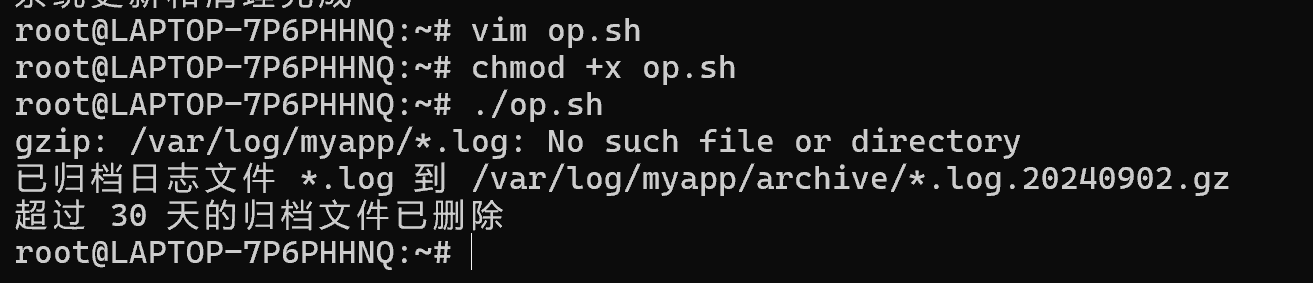
\includegraphics[width=\textwidth]{17} % 确保文件名正确
    \caption{效果展示}
  
  \end{figure}
\end{itemize}
\end{enumerate}
%1.1.17超链接==================================================%

%1.1.18积分图像==================================================%

%1.1.19文字结点==================================================%


%1.1.20循环==================================================%














%1.2git=========================================================================%
  \subsection{vim}
  {\color{blue}vim命令展示}




%1.2.1新建 Git 仓库并克隆==================================================%
\subsubsection{安装并配置插件:ctrlp.vim}

\begin{enumerate}
  \item 安装并配置插件:ctrlp.vim
  \begin{itemize}
  \item 命令展示
  \begin{verbatim}
 #1.创建插件目录:
mkdir -p ~/.vim/pack/vendor/start
#2.下载插件:
cd ~/.vim/pack/vendor/start
git clone https://github.com/ctrlpvim/ctrlp.vim
#3.阅读文档,打开 Vim
使用 :h ctrlp 阅读 ctrlp.vim 的帮助文档
#4.使用 CtrlP 定位文件:
#导航到一个包含多个文件的项目目录。
#打开 Vim,输入 :CtrlP 启动文件搜索。
#使用界面快速定位和打开文件。
#5.在 ~/.vimrc 中自定义 CtrlP:
在 ~/.vimrc 中添加以下行,以通过 Ctrl-P 打开
let mapleader = "\<Space>"
nnoremap <C-P> :CtrlP<CR>


  \end{verbatim}

  \item 效果展示
  \begin{figure}[H]
    \centering
    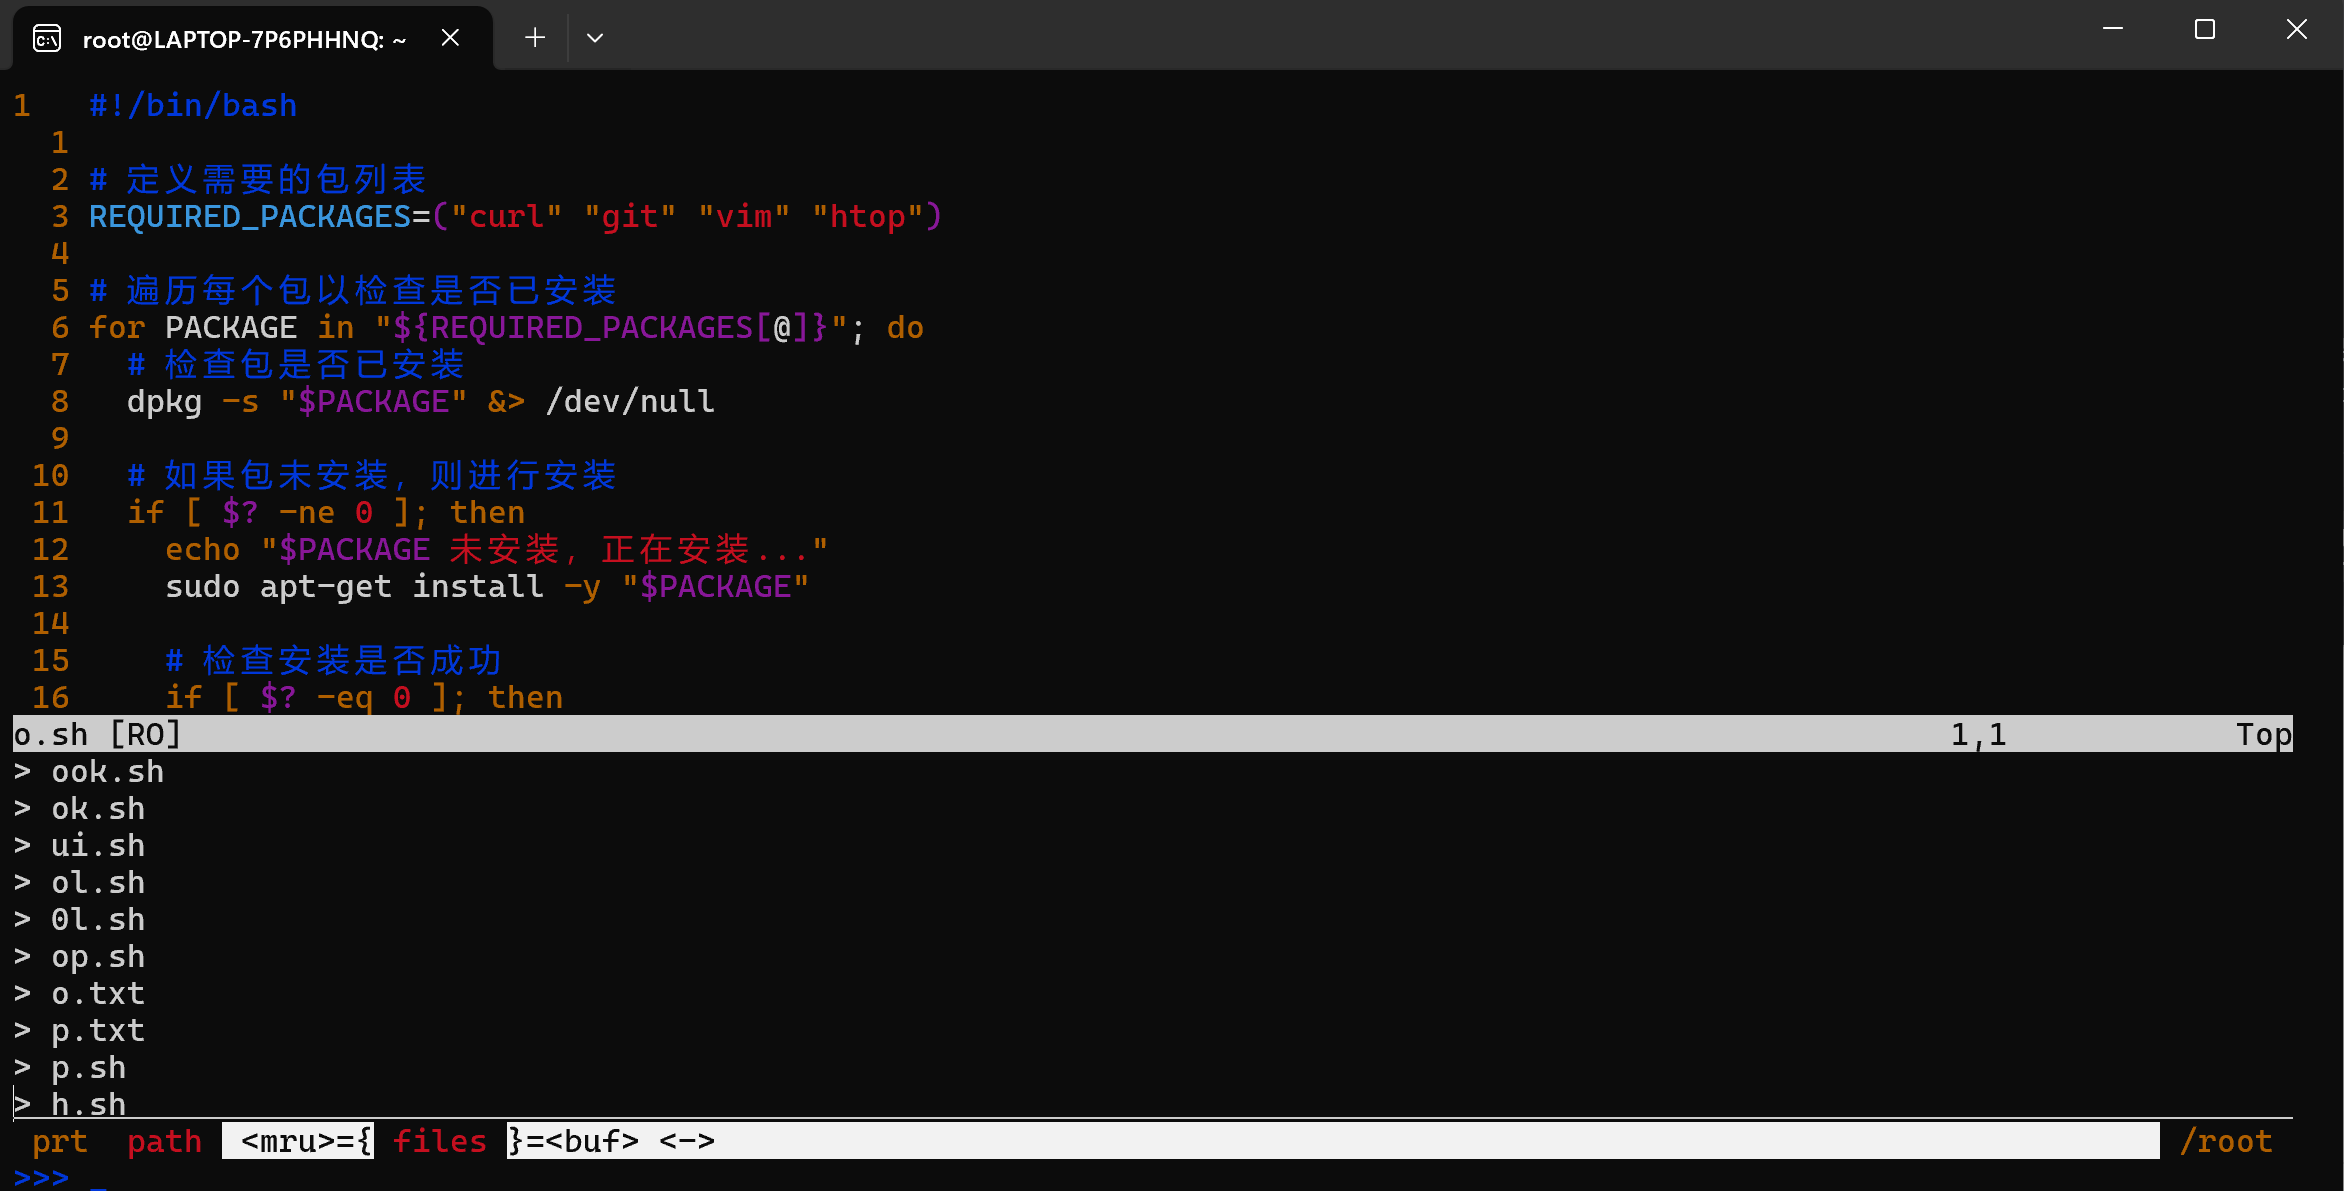
\includegraphics[width=\textwidth]{21} % 确保文件名正确
    \caption{效果展示}
  
  \end{figure}
\end{itemize}
\end{enumerate}


%1.2.2跟踪文件==================================================%
\subsubsection{分屏编辑多个文件}

\begin{enumerate}
  \item 用vim竖直或水平分屏编辑多个文件
  \begin{itemize}
  \item 命令展示
  \begin{verbatim}
 垂直分屏打开新的文件
:vsp filename
水平分屏打开新的文件
:sp filename
 
  \end{verbatim}

  \item 效果展示
  \begin{figure}[H]
    \centering
    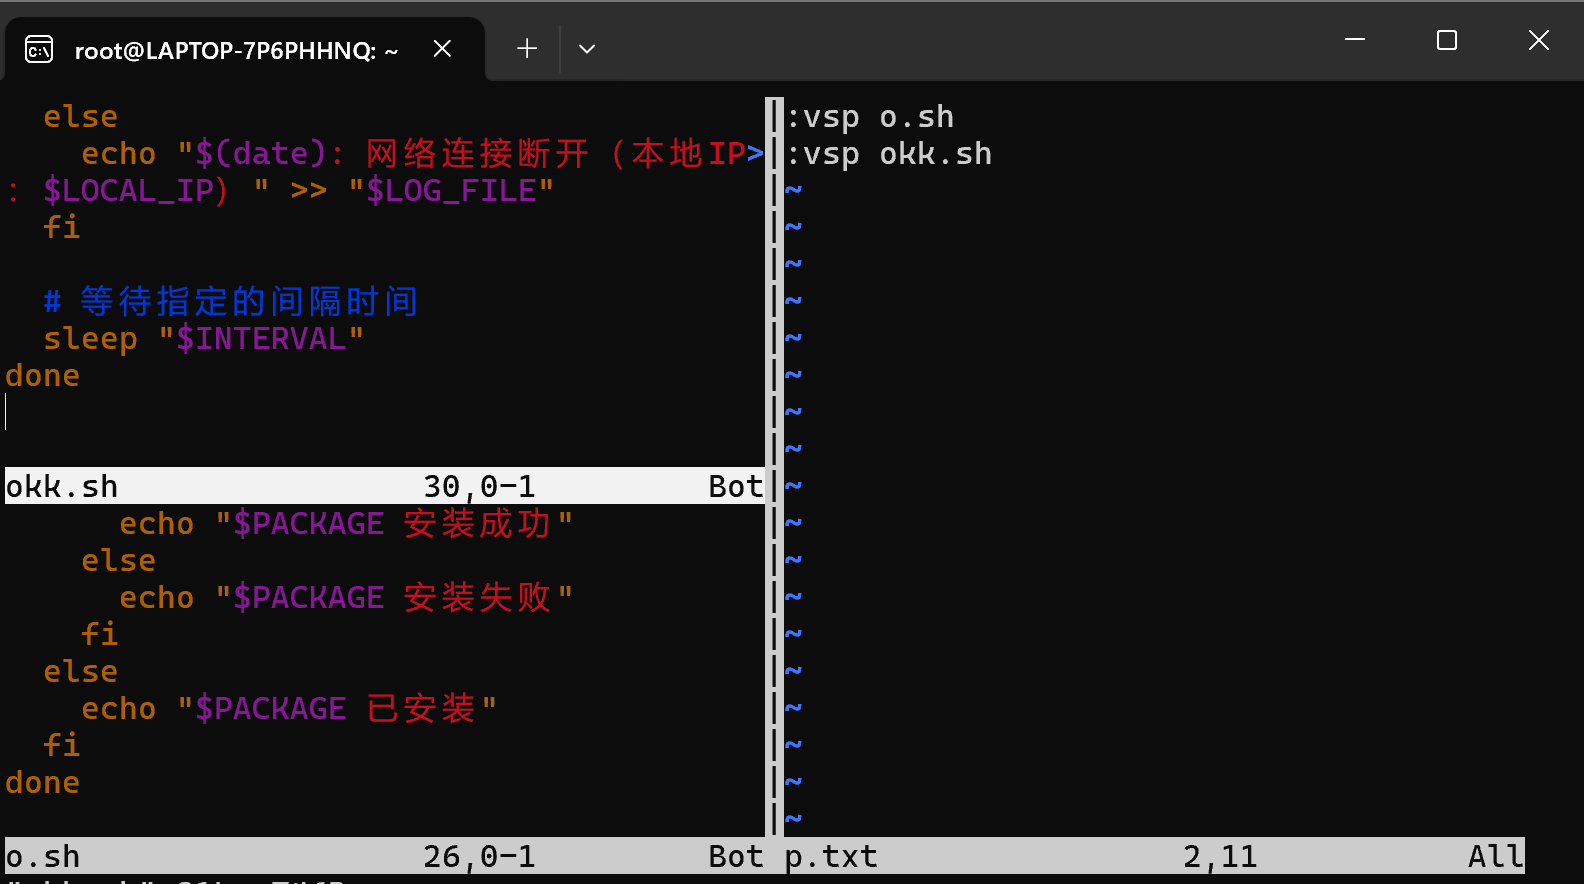
\includegraphics[width=\textwidth]{22} % 确保文件名正确
    \caption{效果展示}
  
  \end{figure}
\end{itemize}
\end{enumerate}

%1.2.3修复最近的提交,但不创建新提交==================================================%
\subsubsection{ 录制宏}

\begin{enumerate}
  \item 在vim中实现多文件搜索与替换
  \begin{itemize}
  \item 命令展示
  \begin{verbatim}
#开始录制宏:
qx  # 这里 x 是寄存器名称,你可以用任何字母代替。
dw  # 删除一个单词
2w            # 向前移动两个单词
iHello<Esc>   #插入 'Hello' 并回到普通模式
#停止录制
q
回放宏
@x

    
  \end{verbatim}

  \item 效果展示
  \begin{figure}[H]
    \centering
    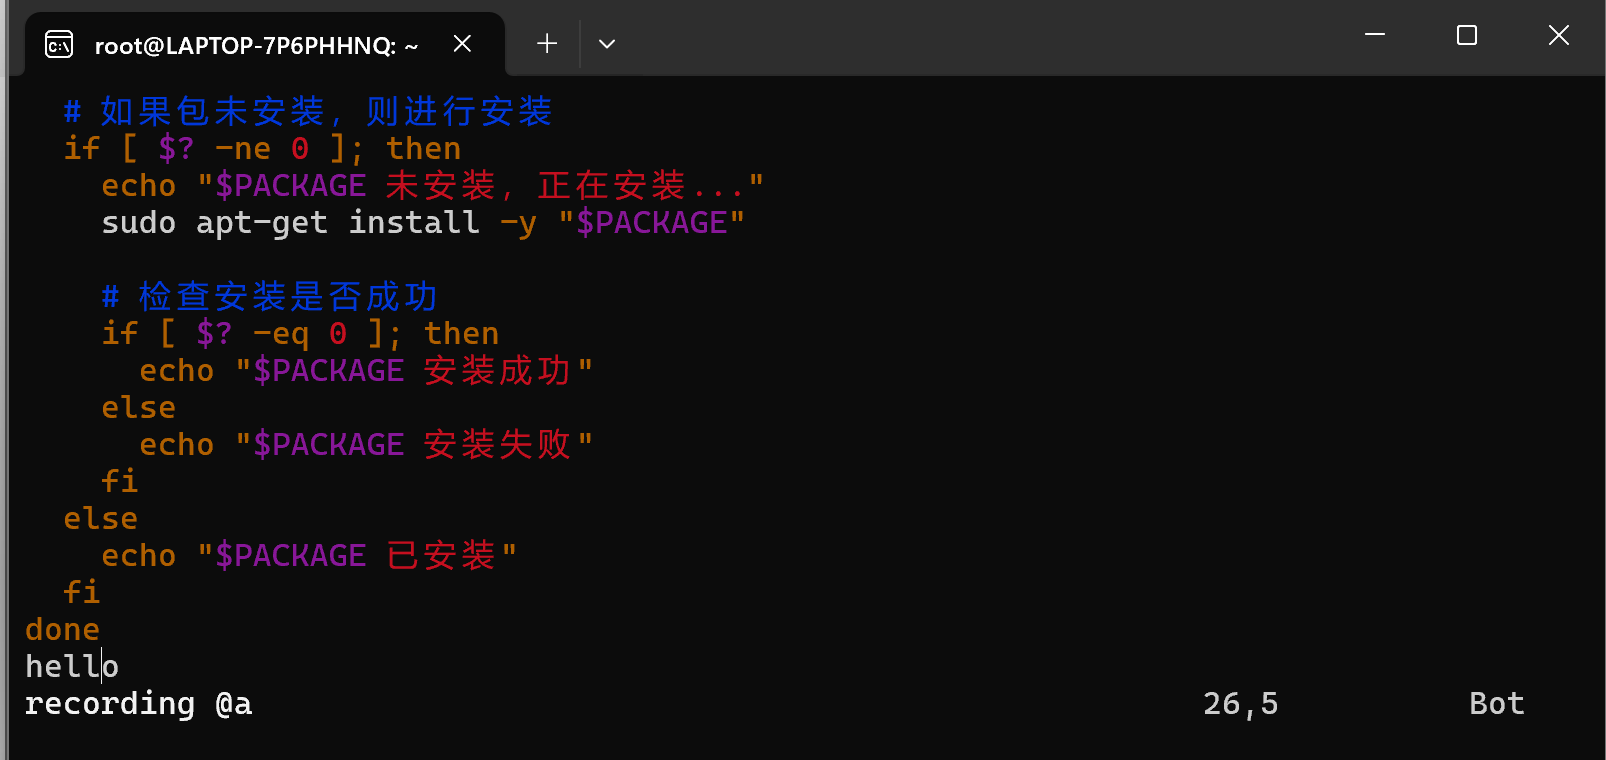
\includegraphics[width=\textwidth]{23} % 确保文件名正确
    \caption{效果展示}
  
  \end{figure}
\end{itemize}
\end{enumerate}

%4=============================================%
\subsubsection{查找和替换历史}

\begin{enumerate}
  \item 使用 Vim 的查找和替换历史
  \begin{itemize}
  \item 命令展示
  \begin{verbatim}
#打开搜索历史窗口
q/

#打开命令行历史窗口
q:


    
  \end{verbatim}

  \item 效果展示
  \begin{figure}[H]
    \centering
    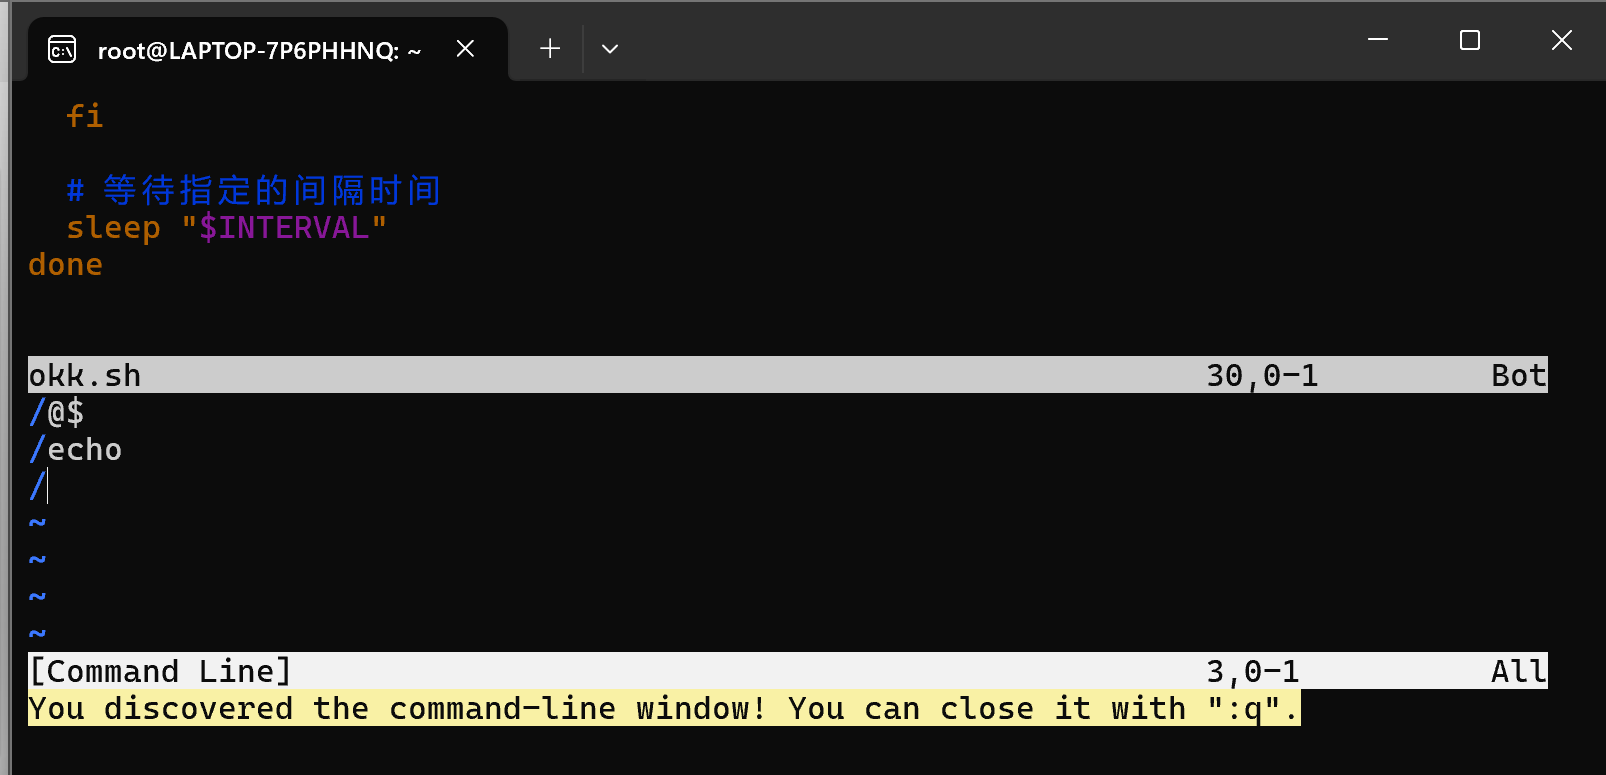
\includegraphics[width=\textwidth]{24} % 确保文件名正确
    \caption{效果展示}
  
  \end{figure}
\end{itemize}
\end{enumerate}
%1.2.5表格==================================================%
\subsubsection{高亮搜索}

\begin{enumerate}
  \item 高亮搜索
  \begin{itemize}
  \item 命令展示
  \begin{verbatim}
#启用搜索高亮
:set hlsearch
#关闭搜索高亮
:set nohlsearch 
#启用增量搜索
:set incsearch 
    
  \end{verbatim}

  \item 效果展示
  \begin{figure}[H]
    \centering
    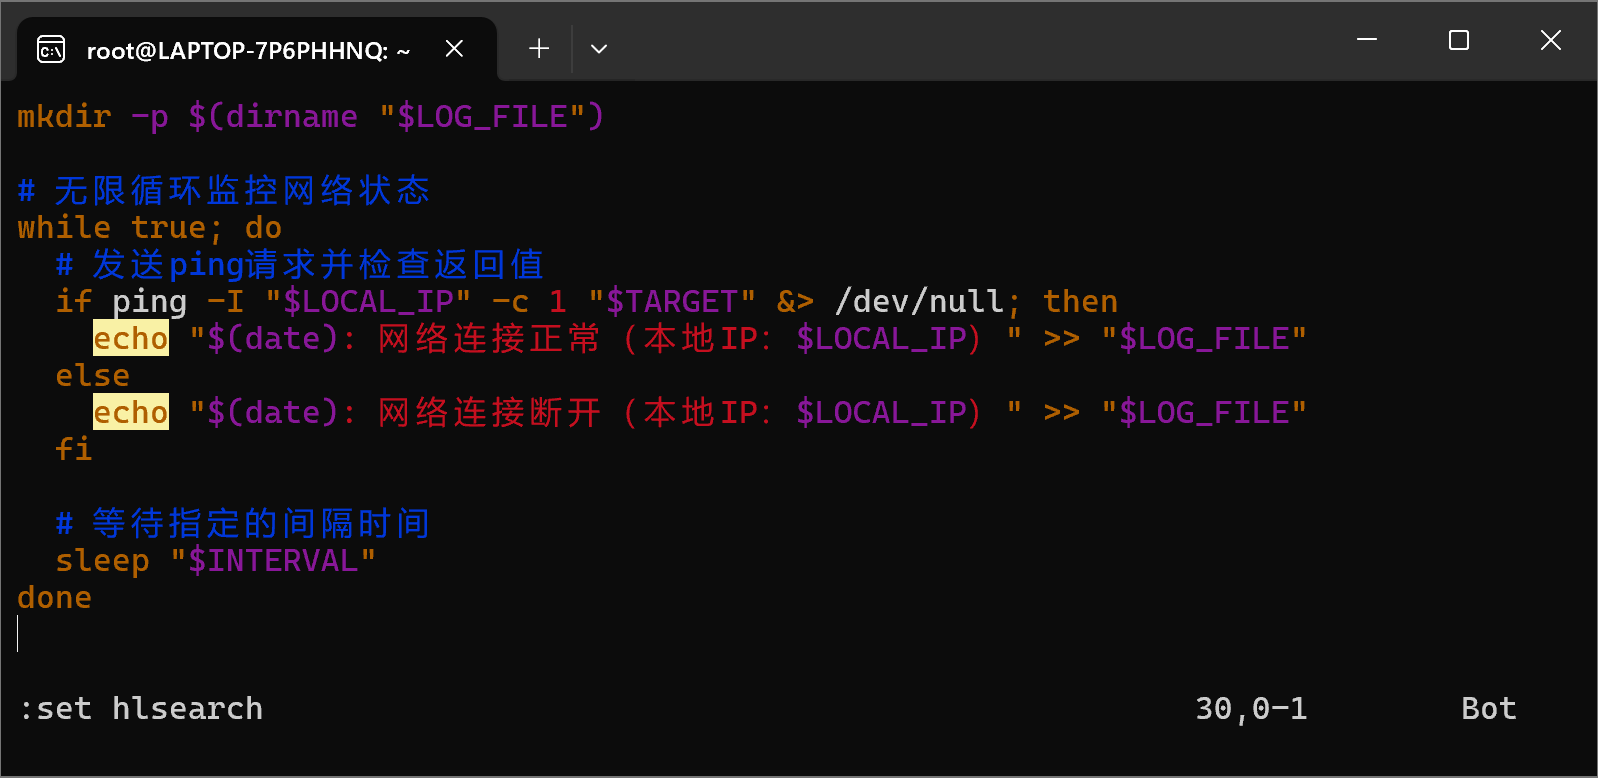
\includegraphics[width=\textwidth]{25} % 确保文件名正确
    \caption{效果展示}
  
  \end{figure}
\end{itemize}
\end{enumerate}
%1.2.7表格==================================================%
\subsubsection{将所有制表符转换为空格}

\begin{enumerate}
  \item 编辑的文件使用制表符缩进,并且要将制表符转换为空格,则需要运行如下vim 命令
  \begin{itemize}
  \item 命令展示
  \begin{verbatim}
:set expandtab
:set tabstop=4
:set shiftwidth=4
:retab

    
  \end{verbatim}

  \item 效果展示
  \begin{figure}[H]
    \centering
    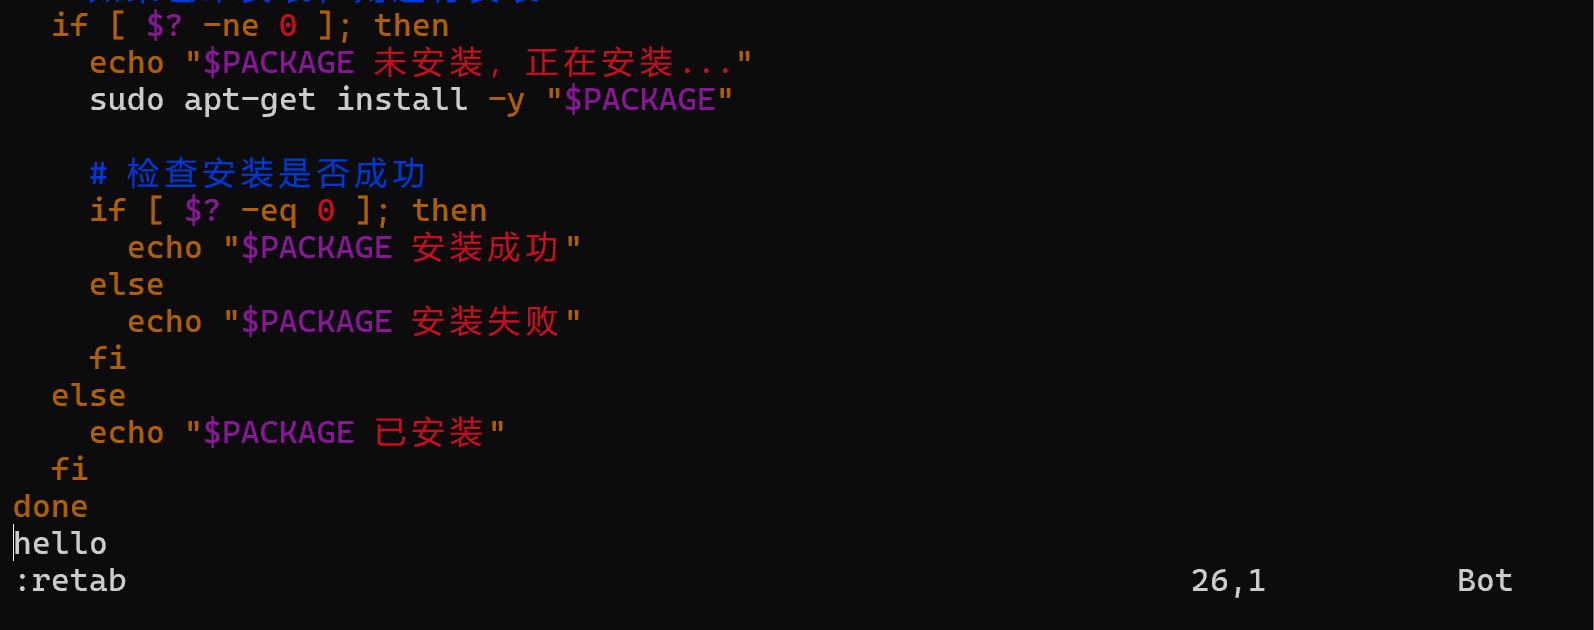
\includegraphics[width=\textwidth]{26} % 确保文件名正确
    \caption{效果展示}
  
  \end{figure}
\end{itemize}
\end{enumerate}
%1.2.8表格==================================================%
\subsubsection{显示行号}

\begin{enumerate}
  \item 在 vim 中显示行号
  \begin{itemize}
  \item 命令展示
  \begin{verbatim}
 #vimrc 中添加以下命令
set number relativenumber

    
  \end{verbatim}

  \item 效果展示
  \begin{figure}[H]
    \centering
    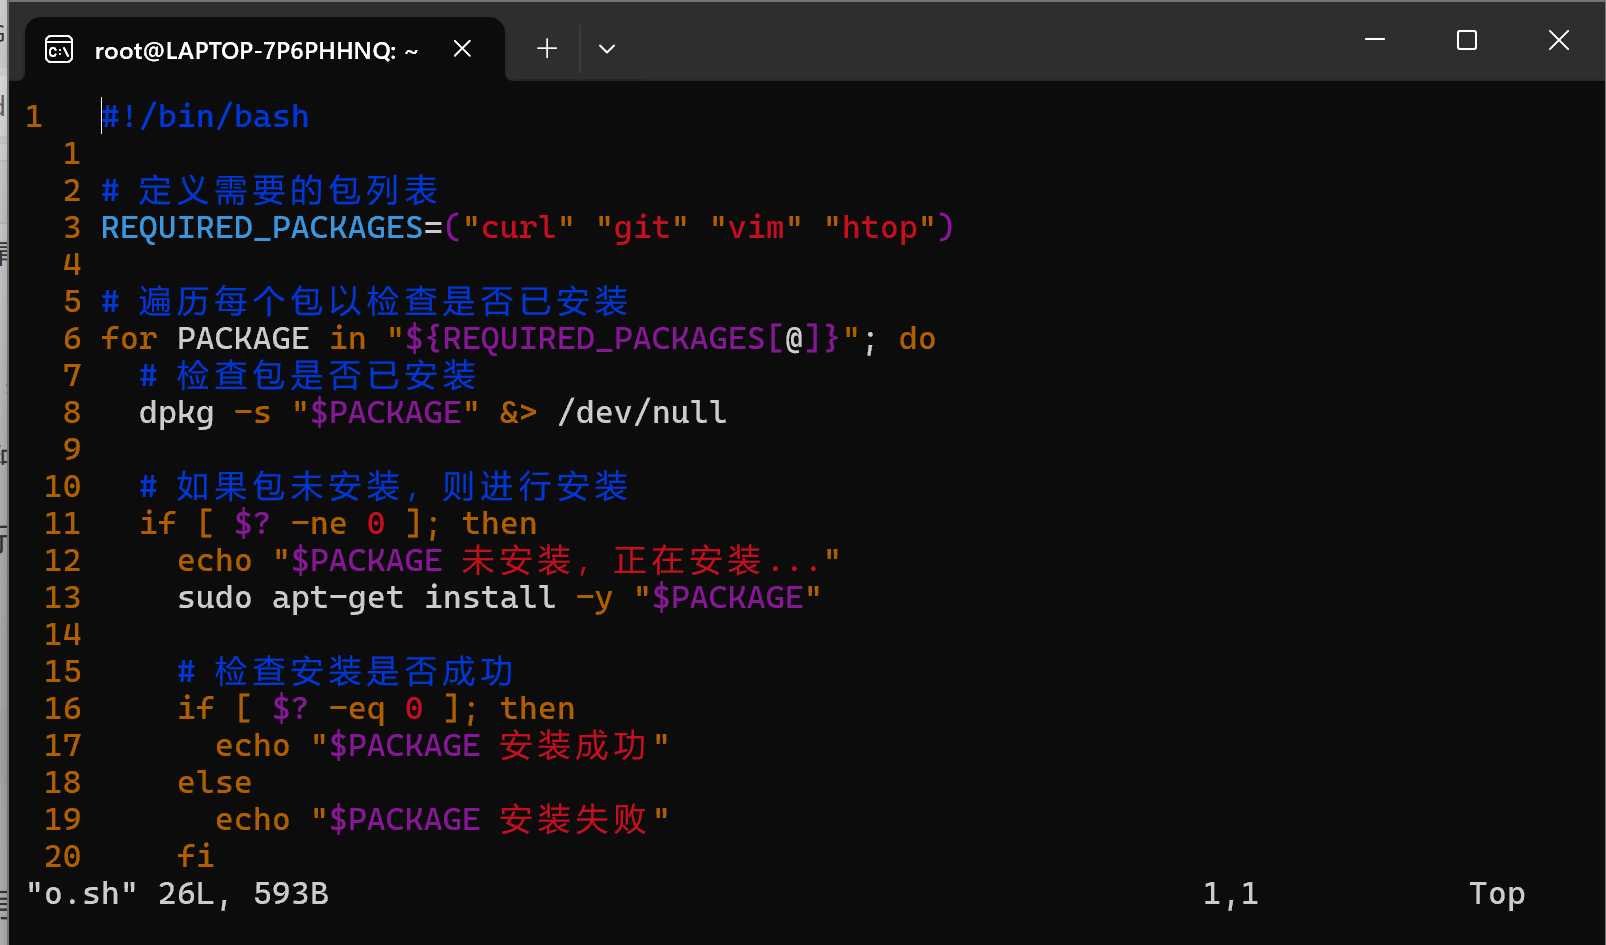
\includegraphics[width=\textwidth]{27} % 确保文件名正确
    \caption{效果展示}
  
  \end{figure}
\end{itemize}
\end{enumerate}
%1.2.9表格==================================================%
\subsubsection{代码折叠}

\begin{enumerate}
  \item 实现代码折叠和收起
输出是彩色的
  \begin{itemize}
  \item 命令展示
  \begin{verbatim}
#在 Vim 配置文件 ~/.vimrc
set foldenable          " 启用折叠功能
set foldmethod=manual   " 设置折叠方法为手动
 zf #创建折叠
 zo #展开折叠
 zc #收起折叠
zM:#折叠所有内容
zR:#展开所有内容。
:set foldmethod=syntax #基于语法折叠代码
  \end{verbatim}

  \item 效果展示
  \begin{figure}[H]
    \centering
    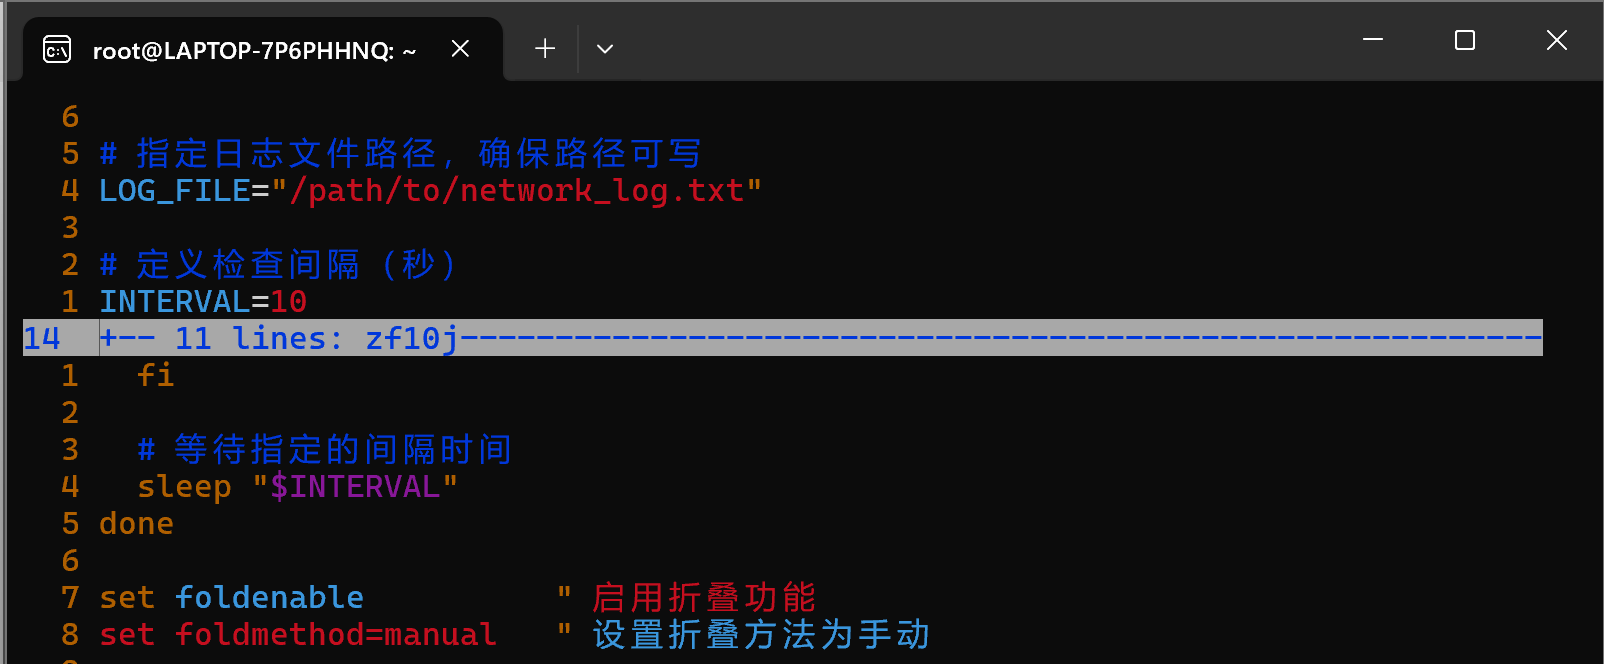
\includegraphics[width=\textwidth]{28} % 确保文件名正确
    \caption{效果展示}
  
  \end{figure}
\end{itemize}
\end{enumerate}
%1.2.10表格==================================================%
\subsubsection{复杂的光标移动}

\begin{enumerate}
  \item 用命令实现复杂的光标移动
  \begin{itemize}
  \item 命令展示
  \begin{verbatim}
  gg     #跳转到文件开头
G        #跳转到文件末尾
{行号}G #跳转到指定行号
:123   #跳转到第123行

    
  \end{verbatim}

  \item 效果展示
  \begin{figure}[H]
    \centering
    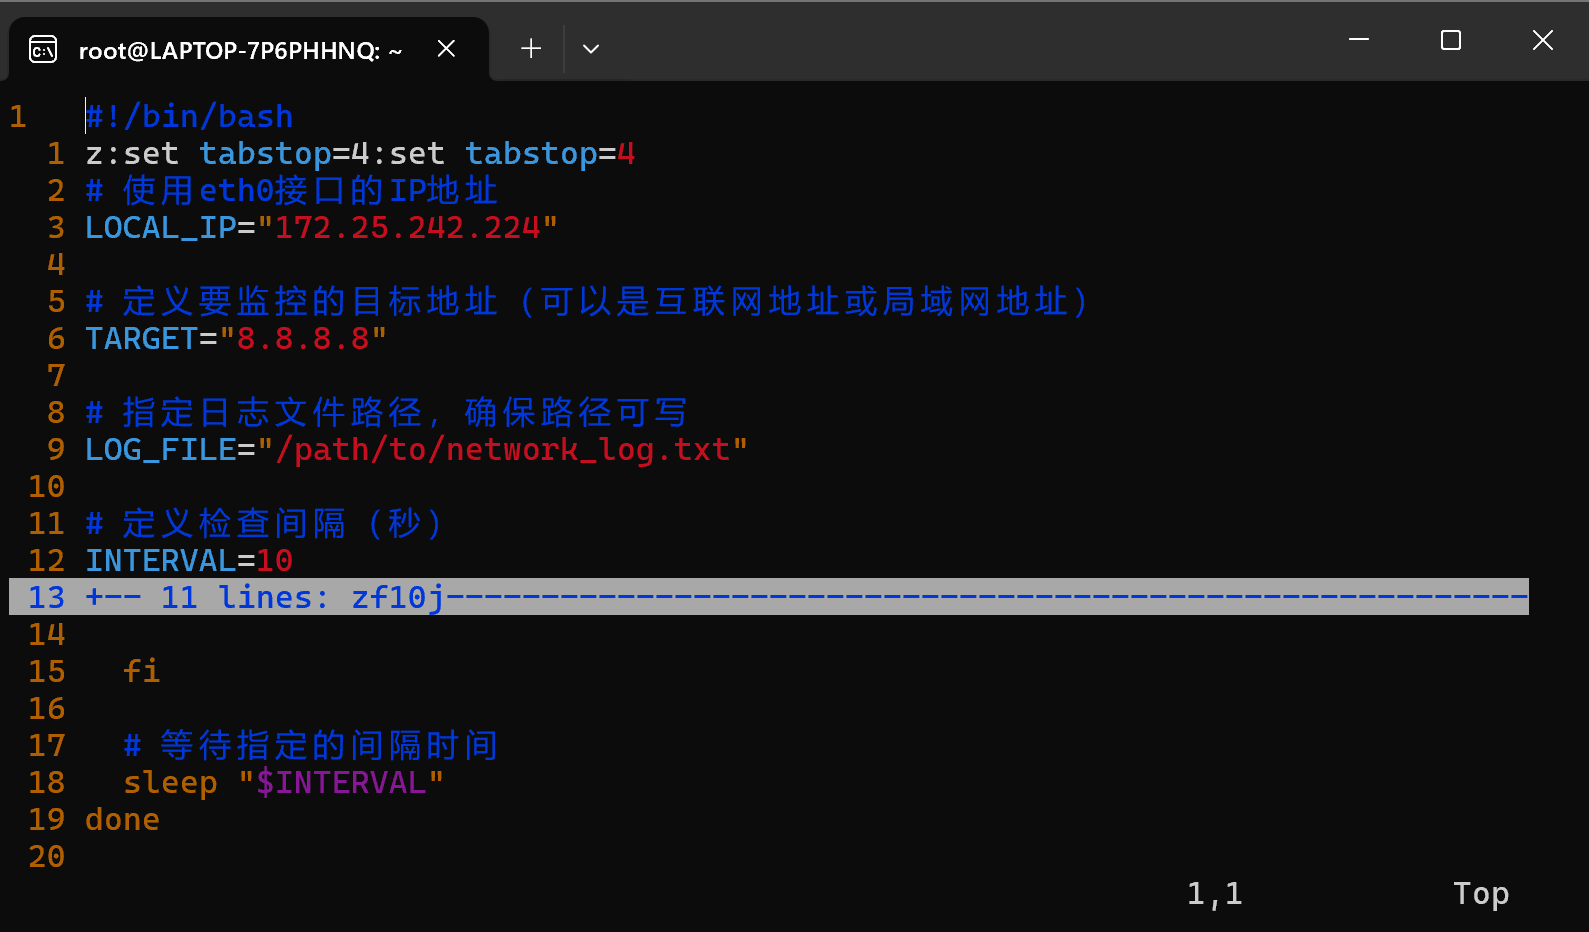
\includegraphics[width=\textwidth]{291}
    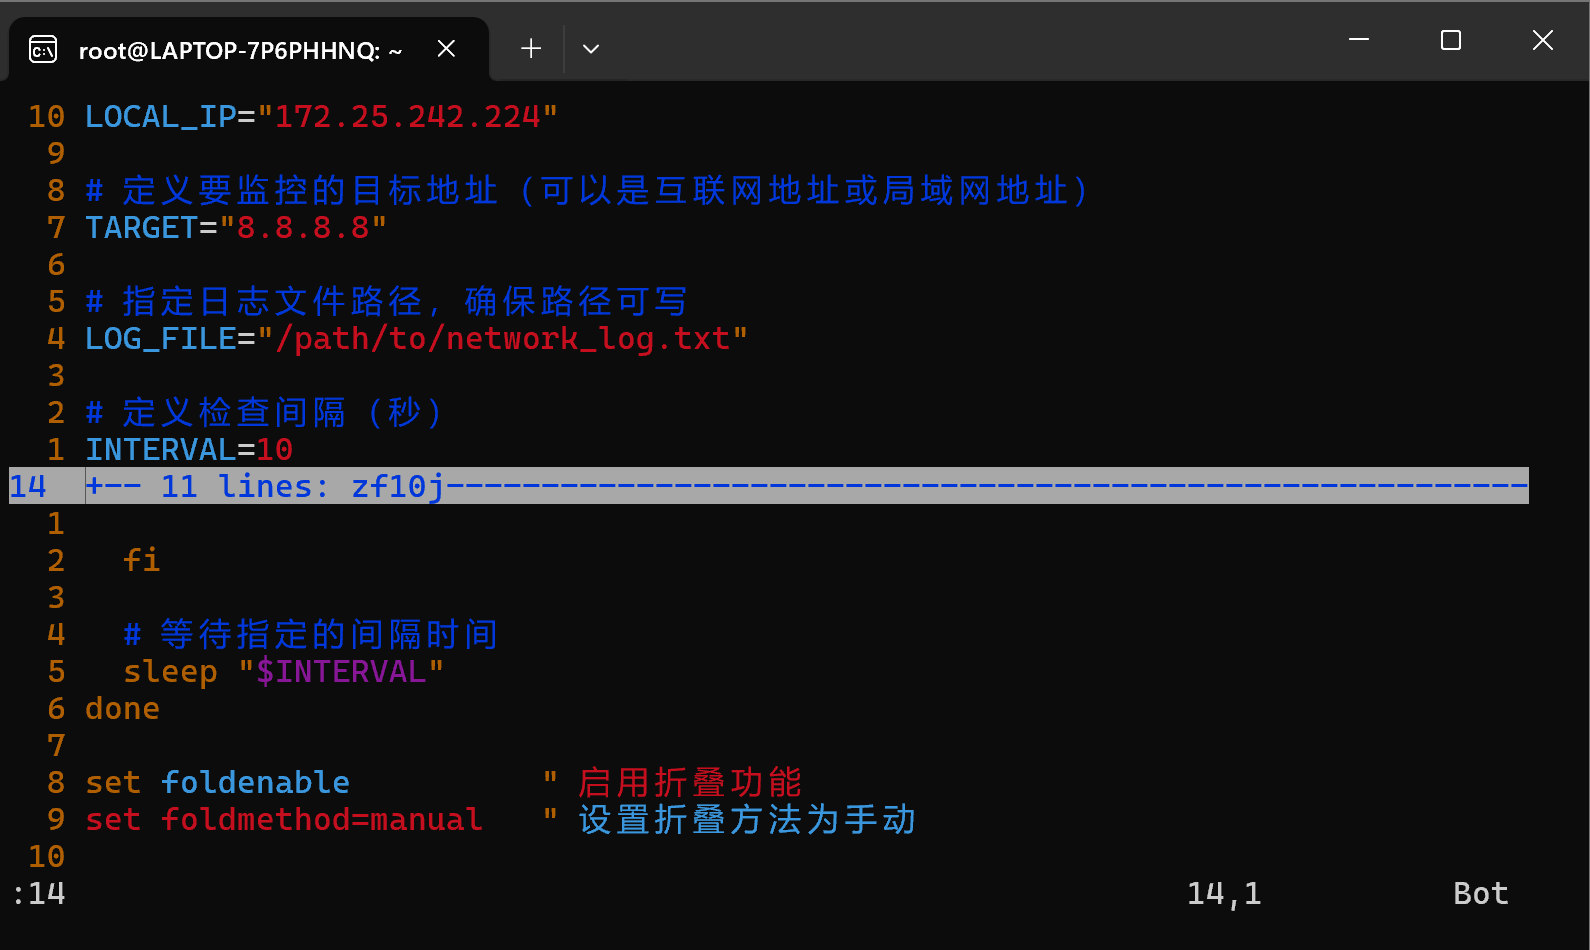
\includegraphics[width=\textwidth]{292}
    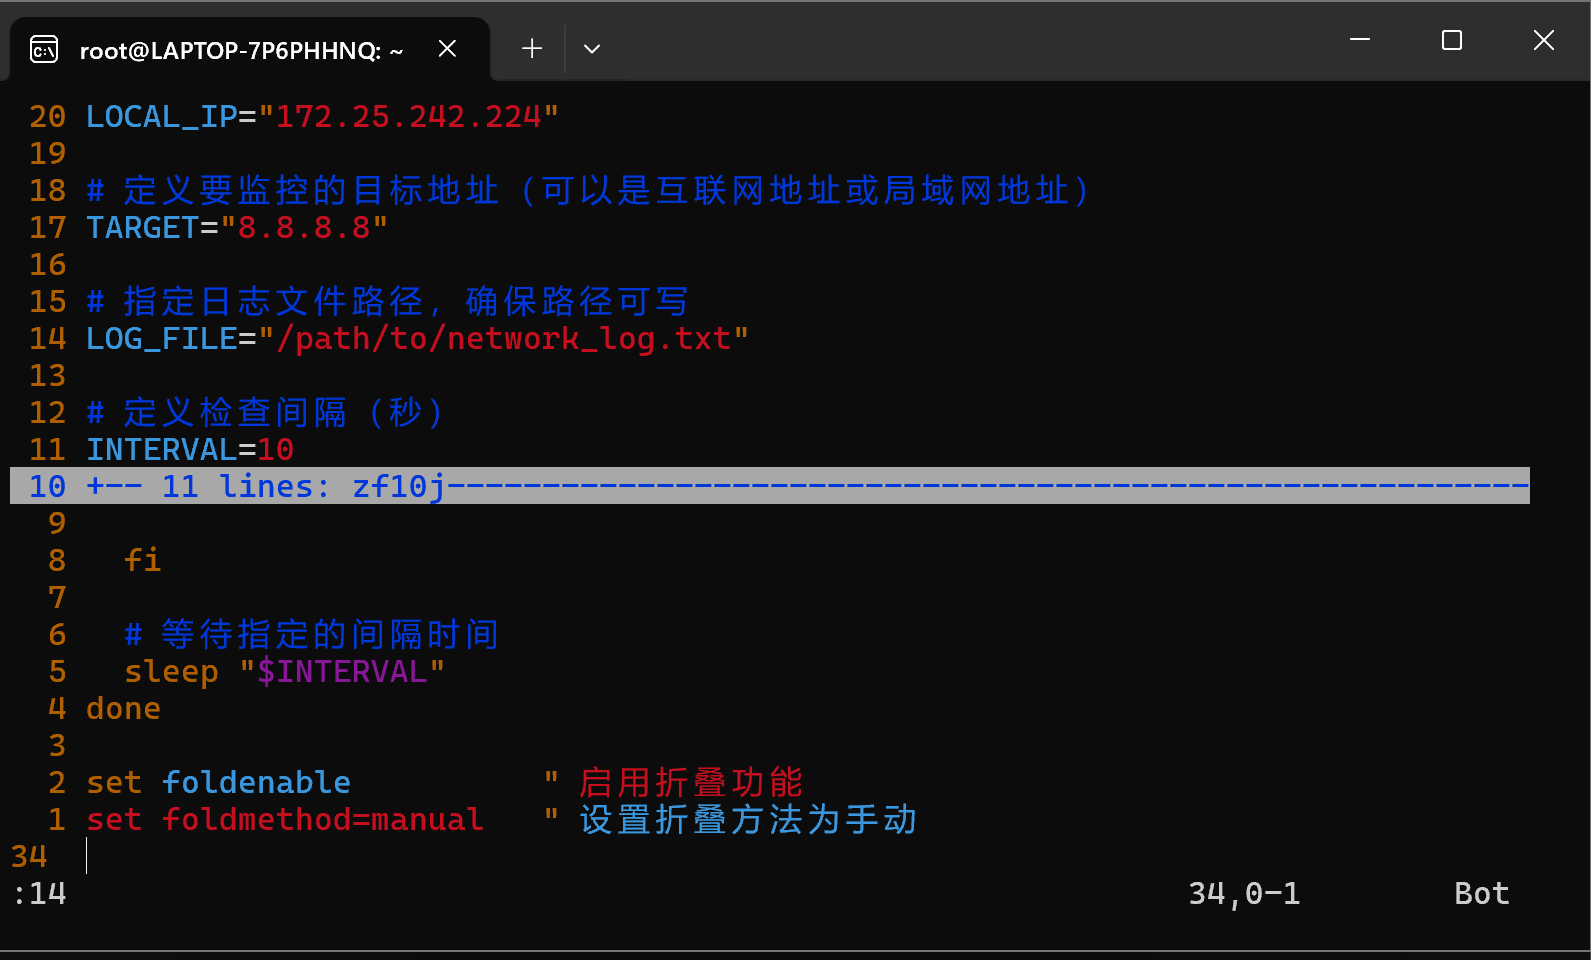
\includegraphics[width=\textwidth]{293} % 确保文件名正确
    \caption{效果展示}
  
  \end{figure}
\end{itemize}
\end{enumerate}

%1.2.12表格==================================================%
\subsubsection{自动补全与代码补全}

\begin{enumerate}
  \item 自动补全与代码补全命令
  \begin{itemize}
  \item 命令展示
  \begin{verbatim}
1.安装支持 Omni Completion 的插件
  Ctrl-n 和 Ctrl-p #在插入模式下进行单词补全
  Ctrl-x Ctrl-f #补全文件名
  Ctrl-x Ctrl-o #补全函数名(需要配置 Omni completion)   
  \end{verbatim}

  \item 效果展示
  \begin{figure}[H]
    \centering
    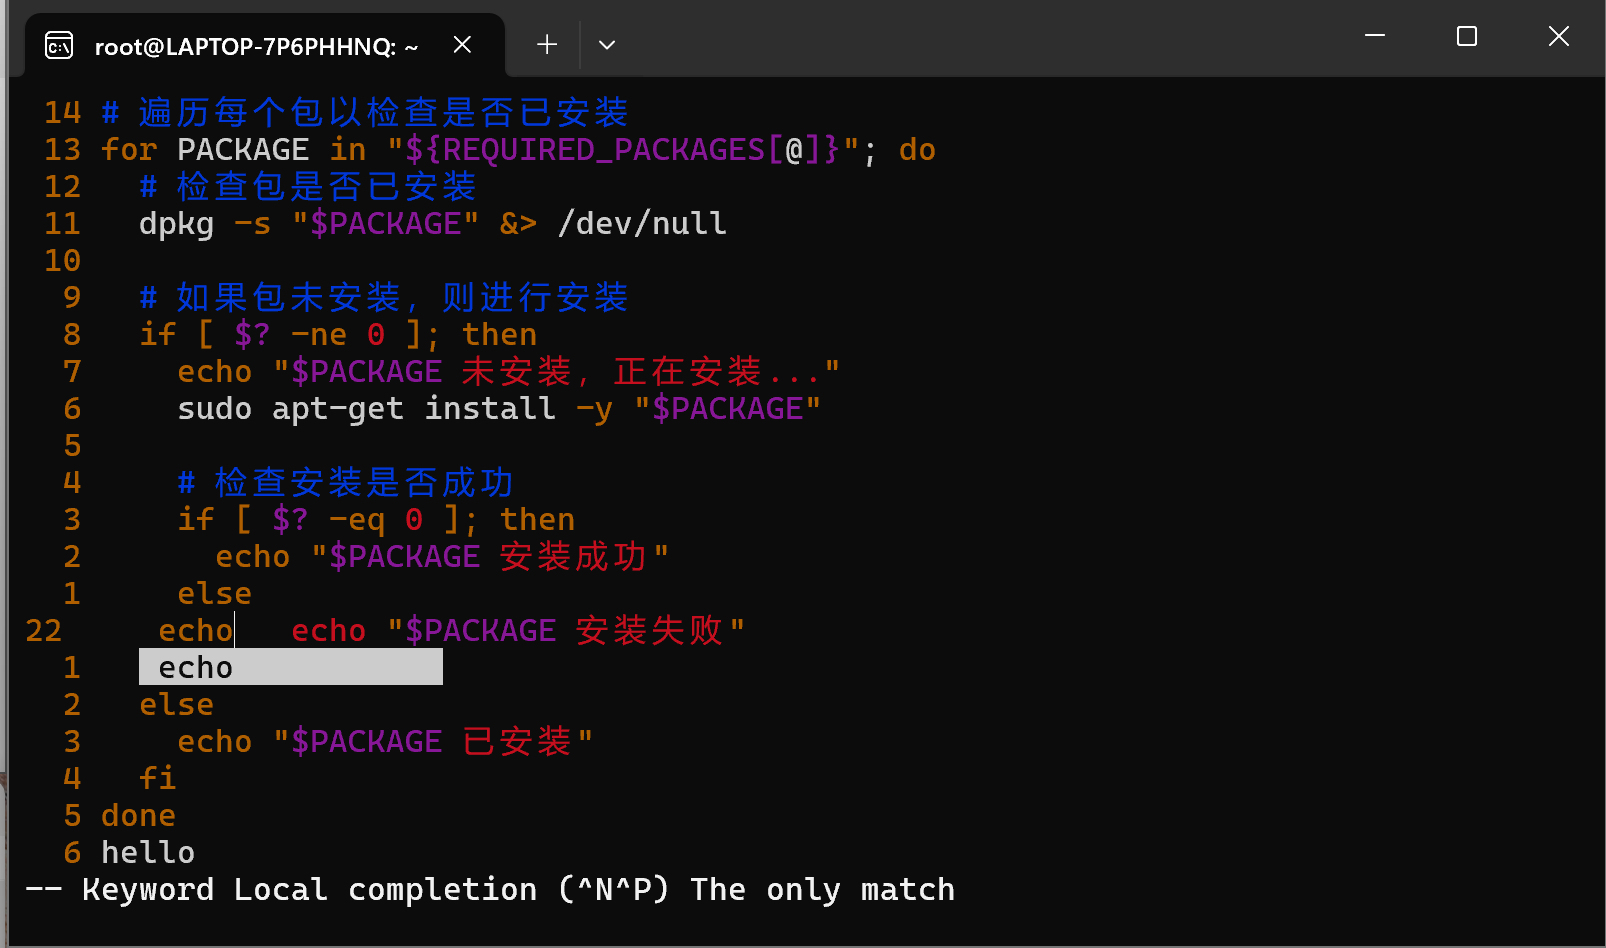
\includegraphics[width=\textwidth]{210} % 确保文件名正确
    \caption{效果展示}
  
  \end{figure}
\end{itemize}
\end{enumerate}

%1.2.13表格==================================================%

%1.2.14表格==================================================%

%1.2.15表格==================================================%

%1.2.16表格==================================================%

%1.2git=========================================================================%
  \subsection{数据整理}
  {\color{blue}数据整理命令展示}

%1.2.1新建 Git 仓库并克隆==================================================%
\subsubsection{从字典中分析单词}

\begin{enumerate}
  \item 找到包含至少三个's'但不以's'结尾的单词,并找出这些单词最后两个字母中最常见的组合。
  \begin{itemize}
  \item 命令展示
  \begin{verbatim}
#1.找到至少包含三个's'的单词:

grep -iE 's.*s.*s' /usr/share/dict/words
#2.排除以's'结尾的单词:

grep -iE 's.*s.*s' /usr/share/dict/words | grep -vi 's$'

#3.提取最后两个字母并统计频率:

grep -iE 's.*s.*s' /usr/share/dict/words | grep -vi 's$' | \
awk '{print substr($0, length($0) - 1)}' | \
sort | uniq -c | sort -nr | head -n 3

  \end{verbatim}

  \item 效果展示
  \begin{figure}[H]
    \centering
    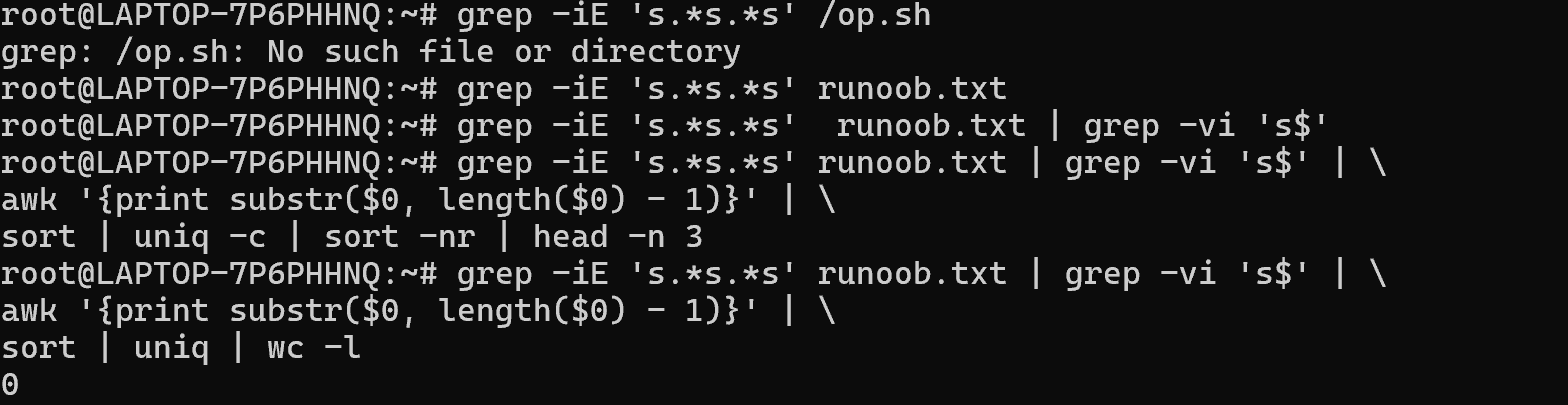
\includegraphics[width=\textwidth]{31} % 确保文件名正确
    \caption{效果展示}
  
  \end{figure}
\end{itemize}
\end{enumerate}


%1.2.2跟踪文件==================================================%
\subsubsection{系统启动时间分析}

\begin{enumerate}
  \item 对最近十次系统启动时间分析
  \begin{itemize}
  \item 命令展示
  \begin{verbatim}
  1. 提取启动时间
# 获取最近十次启动的完成时间
for i in {0..9}; do
    journalctl -b -$i | grep -i 'startup finished' | \
    grep -oP 'in \K[0-9.]+(?=s)' >> boot_times.txt
done
2. 计算统计数据
# 计算平均值、中位数和最大值
awk '{
    times[NR] = $1;
    sum += $1;
    if ($1 > max) max = $1;
}
END {
    # 计算平均值
    avg = sum / NR;
    
    # 计算中位数
    if (NR % 2) {
        median = times[(NR + 1) / 2];
    } else {
        median = (times[NR / 2] + times[NR / 2 + 1]) / 2;
    }
    
    # 输出结果
    printf "Average Boot Time: %.2f seconds\n", avg;
    printf "Median Boot Time: %.2f seconds\n", median;
    printf "Max Boot Time: %.2f seconds\n", max;
}' boot_times.txt

    
  \end{verbatim}

  \item 效果展示
  \begin{figure}[H]
    \centering
    
\includegraphics[width=\textwidth]{32} % 确保文件名正确
    \caption{效果展示}
  
  \end{figure}
\end{itemize}
\end{enumerate}

%1.2.3修复最近的提交,但不创建新提交==================================================%
\subsubsection{唯一启动消息 }

\begin{enumerate}
  \item 从系统启动日志中提取最近的三次启动记录,并找到那些只在其中一次或两次启动记录中出现的日志消息,而不是在所有三次启动记录中都出现的消息。
  \begin{itemize}
  \item 命令展示
  \begin{verbatim}
#1.提取最近三次启动的日志
journalctl -b -0 > boot_log_0.txt
journalctl -b -1 > boot_log_1.txt
journalctl -b -2 > boot_log_2.txt

#2.删除时间戳
sed 's/^[^ ]* //' boot_log_0.txt > clean_boot_log_0.txt
sed 's/^[^ ]* //' boot_log_1.txt > clean_boot_log_1.txt
sed 's/^[^ ]* //' boot_log_2.txt > clean_boot_log_2.txt

#3.合并日志并统计每条消息的出现次数
cat clean_boot_log_0.txt clean_boot_log_1.txt clean_boot_log_2.txt | sort | uniq -c > all_boot_logs.txt

#4.过滤只出现一次或两次的消息
awk '$1 < 3' all_boot_logs.txt > unique_boot_logs.txt


    
  \end{verbatim}

  \item 效果展示
  \begin{figure}[H]
    \centering
    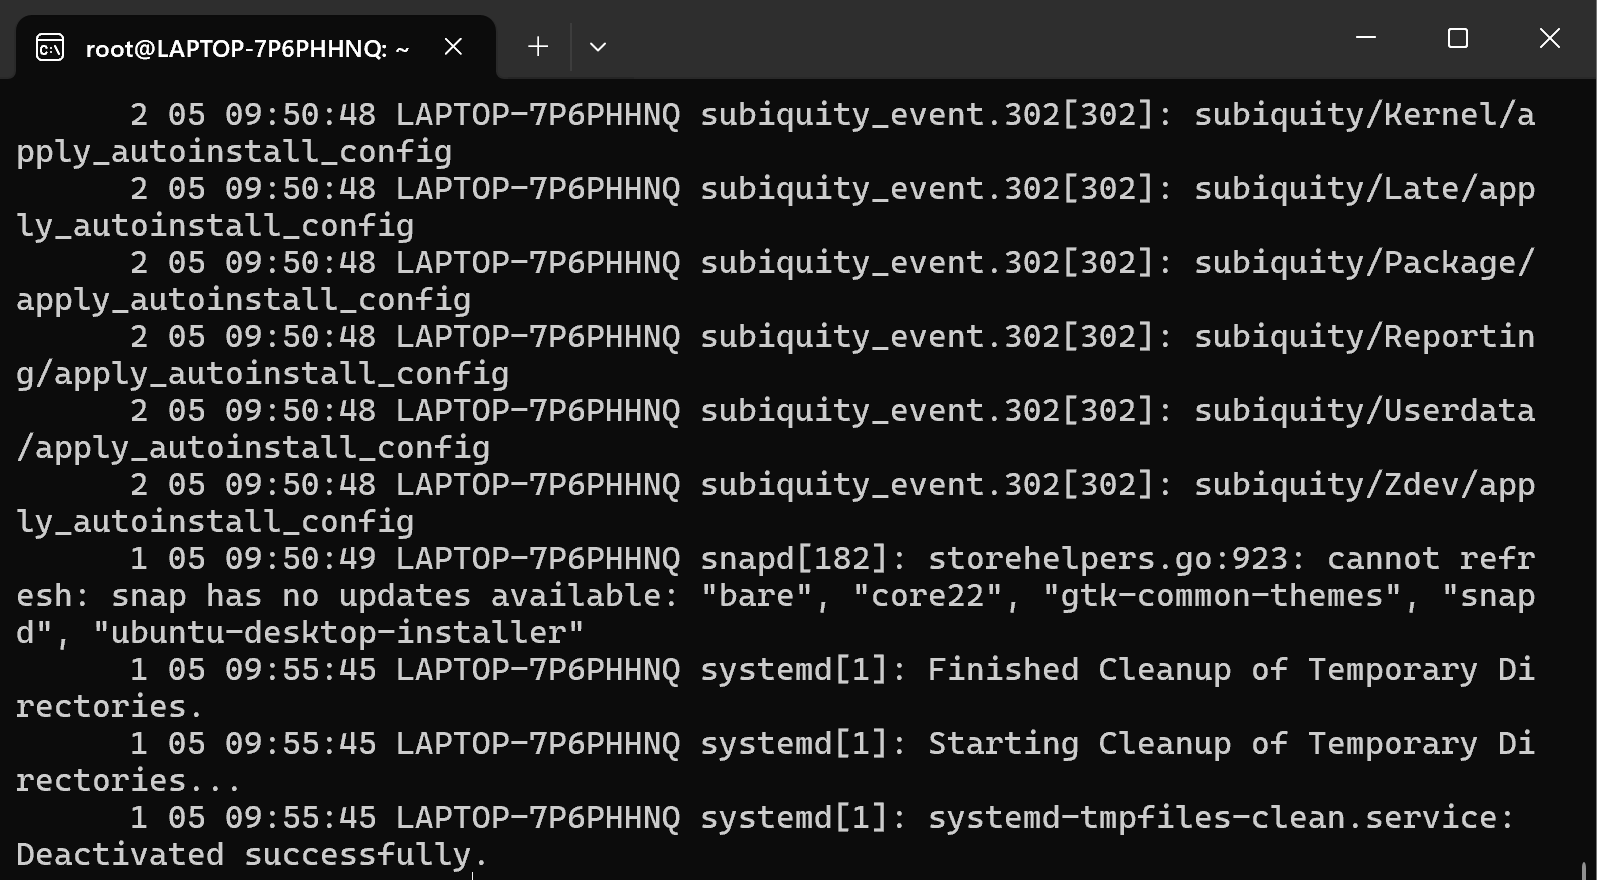
\includegraphics[width=\textwidth]{33} % 确保文件名正确
    \caption{效果展示}
  
  \end{figure}
\end{itemize}
\end{enumerate}
%1.2.3修复最近的提交,但不创建新提交==================================================%
\subsubsection{唯一启动消息 }

\begin{enumerate}
  \item 从系统启动日志中提取最近的三次启动记录,并找到那些只在其中一次或两次启动记录中出现的日志消息,而不是在所有三次启动记录中都出现的消息。
  \begin{itemize}
  \item 命令展示
  \begin{verbatim}
#1.提取最近三次启动的日志
journalctl -b -0 > boot_log_0.txt
journalctl -b -1 > boot_log_1.txt
journalctl -b -2 > boot_log_2.txt

#2.删除时间戳
sed 's/^[^ ]* //' boot_log_0.txt > clean_boot_log_0.txt
sed 's/^[^ ]* //' boot_log_1.txt > clean_boot_log_1.txt
sed 's/^[^ ]* //' boot_log_2.txt > clean_boot_log_2.txt

#3.合并日志并统计每条消息的出现次数
cat clean_boot_log_0.txt clean_boot_log_1.txt clean_boot_log_2.txt | sort | uniq -c > all_boot_logs.txt

#4.过滤只出现一次或两次的消息
awk '$1 < 3' all_boot_logs.txt > unique_boot_logs.txt


    
  \end{verbatim}

  \item 效果展示
  \begin{figure}[H]
    \centering
    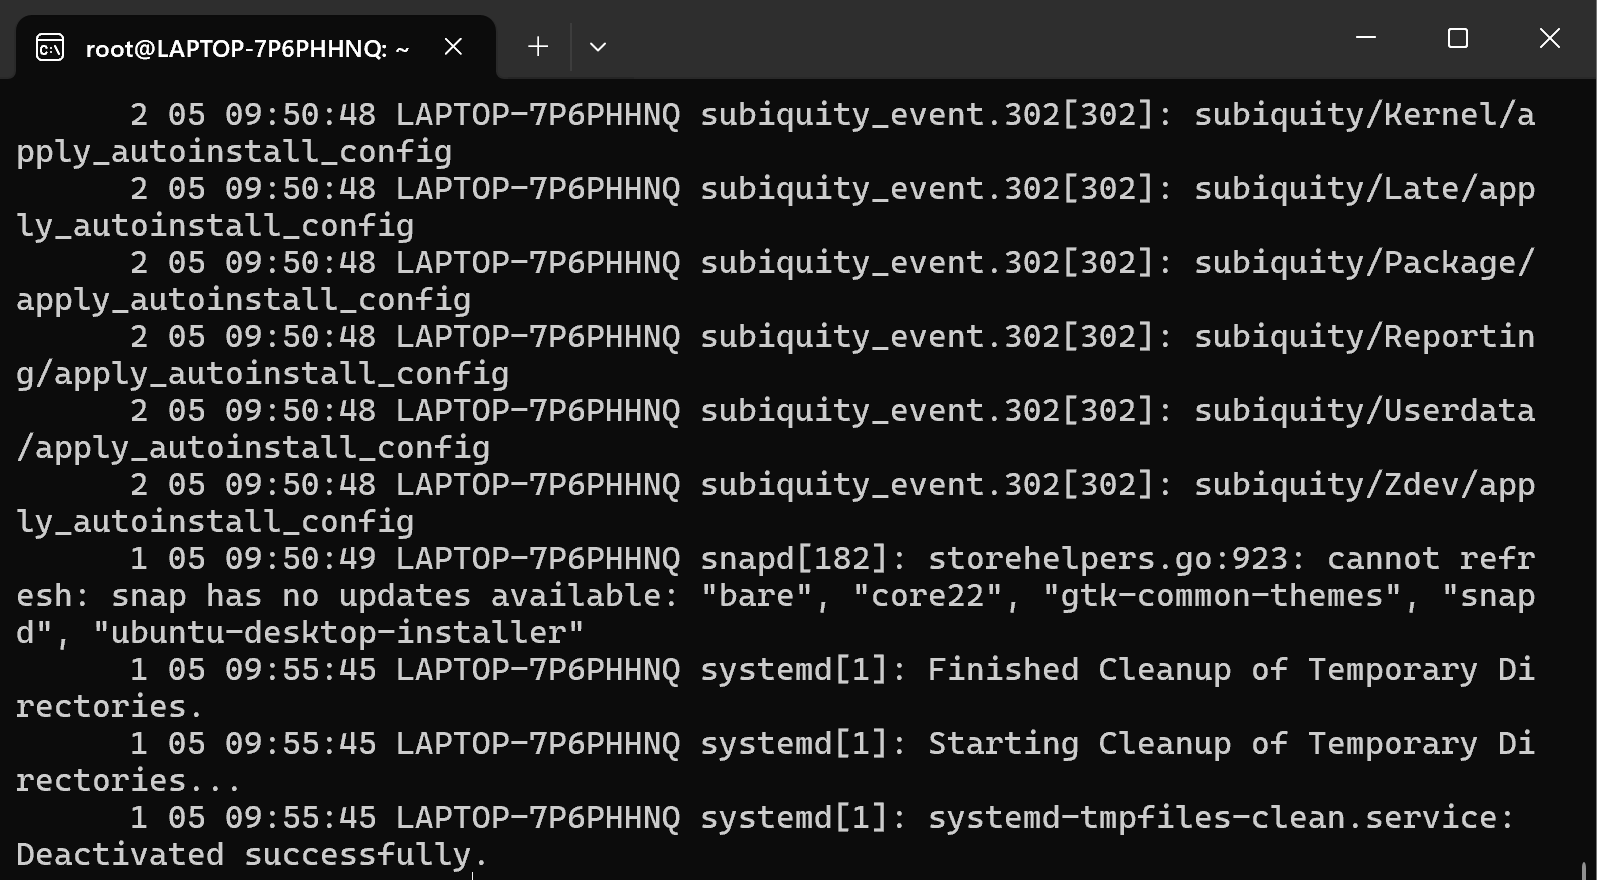
\includegraphics[width=\textwidth]{33} % 确保文件名正确
    \caption{效果展示}
  
  \end{figure}
\end{itemize}
\end{enumerate}























%Shell工具和脚本=========================================================================%
  \section{困难与解决方案}
  \subsection{Shell}
\begin{enumerate}
\item
\begin{itemize}
\item 问题:执行shell脚本时报错 No such file or directory,而目录确实是存在的
\item 解决方案:用vim打开该sh文件,输入:
[plain]//
:set ff//
回车,显示fileformat=dos,重新设置下文件格式://
[plain]//
:set ff=unix//
保存退出://
[plain]//
:wq//
再执行,就可以了
\end{itemize}
\item
\begin{itemize}
\item 问题:unary operator expected
\item 解决方案:用双中括号
\end{itemize}
\item
\begin{itemize}
\item 问题:ret变量不止一行,直接使用:

if [ -z ret]; then//
将报错
\item 解决方案:使用双引号
\end{itemize}

\item
\begin{itemize}
\item 问题:Shell中压缩和解压文件

\item 解决方案:使用 tar 命令
\end{itemize}
\item
\begin{itemize}
\item 问题:Shell中压缩和解压文件

\item 解决方案:使用 tar 命令//
eg.压缩:tar -czvf archive.tar.gz /path/to/director//
解压:tar -xzvf archive.tar.gz
\end{itemize}
\end{enumerate}


\subsection{vim}
\begin{enumerate}
\item
\begin{itemize}
\item 问题:如何在Vim中撤销上一步操作
\item 解决方案:在命令模式下按 u 可以撤销上一次编辑操作。按 Ctrl+R 可以重做
\end{itemize}
\item
\begin{itemize}
\item 问题: Vim中编辑多个文件
\item 解决方案:使用 :n 和 :p 在文件间切换。可以通过 vim file1 file2 启动。:bnext 和 :bprev 也可以用于在缓冲区中导航
\end{itemize}

\item
\begin{itemize}
\item 问题:如何在Vim中使用插件管理器
\item 解决方案:命使用插件管理器如 Vundle 或 vim-plug//
eg.在 ~/.vimrc 中添加://
call plug begin('~/.vim/plugged')//
Plug 'tpope/vim-sensible'//
call plug end()//
在Vim中运行 :PlugInstall 安装插件。

 \end{itemize}
\end{enumerate}




%Shell工具和脚本=========================================================================%
  \section{心得体会}
\begin{itemize}
  \item Shell(尤其是Bash)是Linux和Unix系统管理员及开发者的得力助手。通过Shell脚本,我们可以自动化许多重复性任务,从系统维护到复杂的数据处理工作。Shell提供了强大的命令行工具,如 grep、awk、sed、find 等,这些工具可以组合使用,以高效地处理各种任务。优点:Shell脚本可以大大简化日常任务,减少手动操作的时间。缺点Shell脚本的调试相对困难,特别是当脚本变得复杂时,而且不同的Shell(如Bash、Zsh、Fish)和不同的操作系统(如Linux、macOS)可能存在兼容性问题\\
  \item Vim是不同以往的文本编辑器,打开了键盘工作模式的新大门,缺点Vim的命令和操作模式需要时间学习和适应,且配置文件也不容易,优点通过模式切换和快捷键操作,让文本输入更加连贯,解放鼠标。
   \item 数据整理,十分实用但是上手不是很容易,但是在实际应用中比较有价值。

  \item 学习和使用 Shell 和 Vim 是一段非常有益的经历。我认识到Shell 和 Vim 是两个非常有价值的工具,它们不仅可以提高了工作效率,也让我更深入地理解了 Linux 环境的强大之处。
  \end{itemize}

  \section{github网址}
\href{https://github.com/KeepingMoving/work1.git}{GitHub仓库}
https://github.com/KeepingMoving/work1.git
 










\end{document}